% ------------------------------------------------------------------------
% abnTeX2: Projeto em conformidade com ABNT
% ------------------------------------------------------------------------
\documentclass[
	12pt,
	openright,
	oneside,
	a4paper,
	brazil
]{abntex2}

% ----------------------------------------------------------
% PACOTES
% ----------------------------------------------------------
\usepackage{lmodern}
\usepackage[T1]{fontenc}
\usepackage[utf8]{inputenc}
\usepackage{indentfirst}
\usepackage{color}
\usepackage{graphicx}
\usepackage{microtype}
\usepackage{fancyhdr}
\usepackage[brazilian,hyperpageref]{backref}
\usepackage[alf]{abntex2cite}
\usepackage{hyperref}
\usepackage{multirow}

% ----------------------------------------------------------
% CONFIGURAÇÕES DE PACOTES
% ----------------------------------------------------------
\renewcommand{\backrefpagesname}{Citado na(s) página(s):~}
\renewcommand{\backref}{}
\renewcommand*{\backrefalt}[4]{
	\ifcase #1 Nenhuma citação no texto.%
	\or Citado na página #2.%
	\else Citado #1 vezes nas páginas #2.%
	\fi}
\renewcommand\thesection{\arabic{section}}

% ---
% Informações para CAPA e FOLHA DE ROSTO
% ---
\titulo{Desenvolvimento de um Dashboard para o Monitoramento e Acompanhamento Contínuo de Projetos em Fábricas de Software Acadêmicas}
\autor{Danrley Willyan da Silva Pereira (RGM 42570166)}
\orientador{Kerlla de Souza Luz}
\local{Brasília}
\data{2026}
\instituicao{
  Centro Universitário do Distrito Federal (UDF)\\
  Curso de Ciência da Computação\\
  Programa de Iniciação Tecnol\'{o}gica
}
\tipotrabalho{Artigo de Pesquisa}
\preambulo{Artigo resultante do Programa Institucional de Bolsas de Iniciação Tecnológica \& Inovação (PIBIT) 2025--2026 do Centro Universitário do Distrito Federal (UDF).}

% HYPERSETUP
\makeatletter
\hypersetup{
	pdftitle={\@title},
	pdfauthor={\@author},
	pdfsubject={\imprimirpreambulo},
	pdfkeywords={Dashboard}{F\'{a}brica de Software Acad\^{e}mica}{M\'{e}tricas}{KPIs}{Arquitetura Medalh\~{a}o},
	colorlinks=true,
	linkcolor=blue,
	citecolor=blue,
	filecolor=magenta,
	urlcolor=blue,
}
\makeatother

% ---
% Quadros (se necessário)
% ---
\newcommand{\quadroname}{Quadro}
\newcommand{\listofquadrosname}{Lista de quadros}
\newfloat[chapter]{quadro}{loq}{\quadroname}
\newlistof{listofquadros}{loq}{\listofquadrosname}
\newlistentry{quadro}{loq}{0}
\setfloatadjustment{quadro}{\centering}
\counterwithout{quadro}{chapter}
\renewcommand{\cftquadroname}{\quadroname\space}
\renewcommand*{\cftquadroaftersnum}{\hfill--\hfill}
\setfloatlocations{quadro}{hbtp}

% Espaçamento
\setlength{\parindent}{1.3cm}
\setlength{\parskip}{0.2cm}

\makeindex

% ----
% Início do documento
% ----
\begin{document}
\selectlanguage{brazil}
\frenchspacing

% Folha de rosto
\imprimirfolhaderosto

% ----------------------------------------------------------
% ELEMENTOS PRÉ-TEXTUAIS: RESUMO E ABSTRACT
% ----------------------------------------------------------
\begin{resumo}
Este trabalho apresenta o \textbf{Dashboard de Monitoramento} --- uma plataforma \textit{open source full-stack} para monitoramento contínuo de projetos em \textit{Fábricas de Software Acadêmicas}, co-desenvolvida em colaboração com a \textbf{Dra.\ Carla Rocha} (UnB). A plataforma combina \textbf{métricas técnicas} (commits, \textit{pull requests}, \textit{issues}, \textit{code churn}, tempos) e \textbf{métricas colaborativas} (participação em \textit{reviews}, redes de colaboração, distribuição de contribuições) em \textbf{13+ páginas interativas} com visualizações D3.js e análise por inteligência artificial (Google Gemini). A abordagem metodológica é \textbf{mista} (quanti--qualitativa): dados extraídos da \textbf{API do GitHub} são organizados na \textbf{Arquitetura Medalhão} (Bronze$\rightarrow$Silver$\rightarrow$Gold) e \textbf{triangulados} com evidências qualitativas (Apêndices A e B). O dashboard foi implantado em \textbf{duas instâncias em produção} (UnB e UDF), alcançando \textbf{94\% de cobertura de testes} no frontend e \textbf{otimização de 100x} no pipeline de extração. Dra.\ Carla utilizou o dashboard para \textbf{avaliar seus alunos} ao final do semestre, validando a plataforma em contexto pedagógico real. Distribuído sob \textbf{licença GPL v3.0}, o dashboard opera com \textbf{infraestrutura zero} via GitHub Pages e GitHub Actions, democratizando o acesso a analytics acadêmicos.

\textbf{Palavras-chave:} Dashboard; Fábrica de Software Acadêmica; Métricas; KPIs; Arquitetura Medalhão.
\end{resumo}

\begin{resumo}[Abstract]
\begin{otherlanguage*}{english}
This paper presents an \textit{open-source full-stack} \textbf{dashboard} platform for continuous monitoring of projects in \textit{Academic Software Factories}, co-developed in collaboration with \textbf{Dr.\ Carla Rocha} (UnB). The platform combines \textbf{technical metrics} (commits, pull requests, issues, code churn, lead times) and \textbf{collaboration metrics} (code-review participation, collaboration networks, contribution distribution) across \textbf{13+ interactive pages} with D3.js visualizations and AI-powered analysis (Google Gemini). We adopt a \textbf{mixed-methods} approach: data extracted from the \textbf{GitHub API} is organized in the \textbf{Medallion Architecture} (Bronze$\rightarrow$Silver$\rightarrow$Gold) and \textbf{triangulated} with qualitative evidence (Appendices A and B). The dashboard was deployed in \textbf{two production instances} (UnB and UDF), achieving \textbf{94\% frontend test coverage} and \textbf{100x extraction optimization}. Dr.\ Carla used the dashboard to \textbf{evaluate her students} at the end of the semester, validating the platform in a real pedagogical context. Distributed under \textbf{GPL v3.0}, the dashboard operates with \textbf{zero infrastructure} via GitHub Pages and GitHub Actions, democratizing access to academic analytics.

\textbf{Keywords:} Dashboard; Academic Software Factory; Metrics; KPIs; Medallion Architecture.
\end{otherlanguage*}
\end{resumo}

% Sumário
\pdfbookmark[0]{\contentsname}{toc}
\tableofcontents*
\cleardoublepage

% ----------------------------------------------------------
% ELEMENTOS TEXTUAIS
% ----------------------------------------------------------
\textual

% ===============================
% INTRODUÇÃO
% ===============================
\section{Introdução}

As \textit{Fábricas de Software Acadêmicas} vêm se consolidando como ambientes pedagógicos que aproximam teoria e prática, ao inserir estudantes em projetos reais com práticas e ferramentas utilizadas na indústria \cite{dos2021experiencia,romanha2016modelo,neto2017relato,oliveira2017conduccao,romanha2015fabrica,almeida2006liccoes}. Em tais contextos, a disponibilidade de \textbf{métricas} operacionais e gerenciais é condição para reduzir assimetrias de informação entre docentes, gestores e equipes, apoiar feedback formativo e orientar a melhoria contínua.

Embora plataformas como o GitHub forneçam estatísticas nativas, a literatura indica lacunas de cobertura e padronização para a tomada de decisão educacional, motivando a definição de \textbf{indicadores complementares} e de planos de medição alinhados a objetivos \cite{barbosaIndicadoresConjunto2016,kitchenham2010s}. Em paralelo, estudos e relatos técnicos mostram a viabilidade de pipelines de \textbf{Extração, Transformação e Carga (ETL)} a partir da API do GitHub para alimentar \textbf{dashboards} com visões por projeto, equipe e indivíduo.

Este artigo apresenta o \textbf{Dashboard de Monitoramento} --- uma plataforma \textit{open source full-stack} para monitoramento contínuo de projetos em \textit{Fábricas de Software Acadêmicas}. O dashboard combina \textbf{métricas técnicas} (commits, \textit{pull requests}, \textit{issues}, \textit{churn}, tempos de revisão) e \textbf{métricas colaborativas} (participação em revisões, rede de colaboração e distribuição das contribuições) em 13+ páginas interativas com visualizações D3.js e análise por inteligência artificial. As contribuições são: (i) síntese e implementação de KPIs técnicos e colaborativos para projetos acadêmicos baseados em GitHub; (ii) pipeline de dados completo na Arquitetura Medalhão (Bronze$\rightarrow$Silver$\rightarrow$Gold) com otimização de 100x; (iii) plataforma \textit{full-stack} com 13+ páginas interativas D3.js e módulo de IA; (iv) validação em cenário real --- Dra.\ Carla Rocha (UnB) utilizou o dashboard para avaliar seus alunos.

\noindent
\textbf{Enfoque qualitativo e triangulação.} Além da instrumentação de métricas no GitHub, o estudo incorpora uma vertente qualitativa para interpretar \emph{quando} e \emph{por que} os números mudam. Foram conduzidas entrevistas com o LAPPIS/UnB (FGA) e com membros e professores do LABTECH/UDF. Os principais achados qualitativos estão descritos no \textbf{Apêndice A} (LAPPIS) e no \textbf{Apêndice B} (LABTECH) e orientaram a definição e leitura dos KPIs, evitando interpretações ingênuas de contagens brutas.

\noindent
\textbf{Co-desenvolvimento e validação.} O dashboard foi co-desenvolvido em colaboração com a \textbf{Dra.\ Carla Rocha}, professora de Métodos de Desenvolvimento de Software (MDS) na UnB. Danrley construiu a plataforma e iterou diretamente com Dra.\ Carla para definir quais dados Silver e Gold ela necessitava para acompanhar e avaliar suas turmas. A fábrica de software LabTech do UDF não possuía projeto ativo no segundo semestre de 2025, o que motivou essa colaboração interinstitucional. Ao final do semestre, Dra.\ Carla utilizou o dashboard para avaliar seus alunos, validando a plataforma em contexto pedagógico real. Duas instâncias estão em produção: UnB (\url{https://unb-mds.github.io/2025-2-Squad-01/}) e UDF (\url{https://labtechudf.github.io/CoOps/}).

% ===============================
% REVISÃO DE LITERATURA
% ===============================
\section{Revisão de Literatura}

A revisão organiza-se em três eixos: (i) \textit{Fábricas de Software Acadêmicas} e a demanda por medição; (ii) métricas e indicadores a partir de Git/GitHub; (iii) \textbf{dashboards} e automação da coleta.

\subsection{Fábricas de Software Acadêmicas e a demanda por métricas}
Relatos nacionais indicam ganhos pedagógicos com a imersão dos estudantes em ambientes que simulam o ciclo de vida completo de projetos, mas também apontam desafios recorrentes: baixa visibilidade do status, falta de padronização de indicadores e assimetria de informação entre stakeholders \cite{dos2021experiencia,romanha2016modelo,neto2017relato,oliveira2017conduccao,romanha2015fabrica,almeida2006liccoes}. Essa agenda reforça a necessidade de \textbf{medição sistemática} para planejamento, monitoramento e melhoria.

\subsection{Métricas e indicadores baseados em Git/GitHub}
A plataforma GitHub viabiliza a mensuração de \textbf{atividade de código} (commits, \textit{pull requests}, \textit{issues}, revisões) e de \textbf{derivações gerenciais} (tempos, taxas, distribuição de trabalho). Em contexto educacional, há evidência do uso de métricas Git para avaliar contribuições individuais e de equipes, como frequência de commits, \textit{code churn}, PRs e desigualdade de contribuição (e.g., concentração) \cite{hamer2021using}. Para que sejam acionáveis, indicadores devem ser \textbf{complementares} aos nativos do GitHub e definidos em planos de medição claros (objetivo, fonte, periodicidade, responsabilidades) \cite{barbosaIndicadoresConjunto2016,kitchenham2010s}.

\subsection{Dashboards e automação de coleta}
Experiências com \textbf{ETL} a partir da API do GitHub mostram a construção de \textbf{painéis gerenciais} que agregam métricas por repositório, período e colaborador. Em ambientes ágeis, ferramentas de monitoramento enfatizam integrações automáticas, periodicidade de medição e visualizações que facilitam inspeção e adaptação \cite{ozkan2019agile,temitope2020software,dos2020usoTrello}.

\subsection{Síntese de KPIs a partir da literatura}

A literatura sobre \textbf{co-desenvolvimento} acadêmico-industrial \cite{jarvela2018collaboration,bjerregaard2021lessons} enfatiza a importância de métricas que capturem não apenas progresso técnico, mas também \textbf{dinâmicas de colaboração} e \textbf{coordenação temporal} \cite{franssen2019cogs}. Em contextos acadêmicos, isto se traduz na necessidade de indicadores que reflitam tanto aprendizagem individual quanto formação de competências colaborativas. A Tabela~\ref{tab:kpis-literatura} resume \textbf{KPIs} alinhados aos objetivos deste estudo (dimensões técnicas e colaborativas) e destaca indicadores derivados dos \textbf{Apêndices A e B} (marcados como "derivado dos Apêndices"), todos operacionalizáveis com dados da API do GitHub.

\begin{table}[htbp]
\centering
\caption{KPIs sintetizados da literatura e dos apêndices para projetos acadêmicos baseados em GitHub}
\label{tab:kpis-literatura}
\renewcommand{\arraystretch}{1.2}
\setlength{\tabcolsep}{4pt}
\footnotesize
\begin{tabular}{p{3.6cm} p{7.6cm} p{3.0cm}}
\hline
\textbf{Categoria} & \textbf{KPI (definição resumida)} & \textbf{Fontes} \\
\hline
Atividade de código & Commits/semana por dev; commits por \textit{sprint} & \cite{hamer2021using} \\
Qualidade/volume & \textit{Code churn} (adições/remoções) por período & \cite{hamer2021using} \\
Fluxo de mudanças & PRs/semana; \textit{lead time} de PR (abertura $\rightarrow$ \textit{merge}) & \cite{hamer2021using,ozkan2019agile} \\
Revisões & Comentários por PR; tempo até primeira resposta & \cite{ozkan2019agile,temitope2020software} \\
Rastreamento de tarefas & Throughput de \textit{issues} (abertas/fechadas); tempo de resolução & \cite{barbosaIndicadoresConjunto2016} \\
Colaboração & \% de membros que revisam código por \textit{sprint} & \cite{ozkan2019agile,temitope2020software} \\
Distribuição do trabalho & Concentração de contribuições (ex.: índice de Gini, top-N\%) & \cite{hamer2021using} \\
Regularidade/ritmo & Dias ativos/semana; lacunas de contribuição & \cite{kitchenham2010s,hamer2021using} \\
Rede de colaboração & Grau/centralidade em grafo (comentários em PR/\textit{issues}) & \cite{hamer2021using} \\
Adoção/ferramentas & Aderência ao fluxo (campos/estados essenciais preenchidos) & \cite{ozkan2019agile,temitope2020software} \\
\hline
\multicolumn{3}{l}{\textbf{KPIs complementares (derivados dos Apêndices A e B; GitHub API):}}\\
\hline
Ritmo inicial & \textbf{Slope\_8w}: inclinação da série semanal de contribuições nas semanas 1--8 & (derivado dos Apêndices) + \cite{kitchenham2010s,hamer2021using} \\
Intenção de participação & \textbf{Clones\_W1--W2}: soma de \textit{clones} no início do semestre & (derivado dos Apêndices); cf.\ \cite{barbosaGeracaoGitHub,oliveira2022plataforma} \\
Papel em rede & \textbf{Centralidade revisor/autor}: grau/intermediação em grafo autor$\leftrightarrow$revisor & \cite{hamer2021using} \\
Cadência individual & \textbf{Regularidade\_semanal}: semanas com $\geq$1 contribuição por membro & \cite{kitchenham2010s,hamer2021using} \\
\hline
\end{tabular}
\end{table}



\subsection{Triangulação quantitativo--qualitativa}
A leitura exclusiva de contagens (como \emph{commits}, \emph{pull requests} ou \emph{issues}) pode ocultar fatores de processo (formação de times, curva de aprendizagem, marcos curriculares). Por isso, este trabalho integra \textbf{triangulação}: séries temporais e agregados são cotejados com evidências qualitativas (entrevistas e observação) documentadas nos \textbf{Apêndices A e B}. Essa integração fortalece a validade das inferências e guia intervenções pedagógicas (p.\,ex., reforço de revisão por pares em semanas críticas).

\subsection{Arquitetura Medalhão e abertura à colaboração}
Adota-se uma arquitetura em camadas para o pipeline de dados, com três \emph{tiers}:
\begin{itemize}
    \item \textbf{Bronze (raw)}: ingestão bruta e \emph{append-only} de dados do GitHub. Preserva o formato original (JSON/eventos), carimbos de tempo e metadados de origem.
    \item \textbf{Silver (cleaned/modelado)}: normalização e homogeneização em modelos tabulares (p.\,ex., \texttt{dim\_repos}, \texttt{dim\_users}, \texttt{fact\_commits}, \texttt{fact\_prs}, \texttt{fact\_issues}, \texttt{fact\_reviews}), com tipos, chaves, padronização temporal e colunas de \emph{linhagem}.
    \item \textbf{Gold (métricas/KPIs)}: camadas analíticas agregadas e prontas para o \emph{dashboard} (p.\,ex., throughput de \emph{issues}, \emph{lead time} de PR, \emph{code churn} semanal, participação em \emph{reviews}).
\end{itemize}

\noindent Esse desenho atende a (i) \textbf{reprodutibilidade e auditoria} (linhagem clara desde a origem) e (ii) \textbf{abertura à colaboração}. Sob \textbf{licença copyleft (GPL3)}, outras Fábricas de Software podem reutilizar o pipeline e \emph{consumir diretamente as camadas Bronze/Silver}.

\subsection{Achados qualitativos (Apêndices A e B) e implicações para KPIs}
Os \textbf{Apêndices A e B} registram evidências úteis para projetar e interpretar os indicadores:
\begin{itemize}
    \item \textbf{Ritmo inicial e engajamento}: o engajamento em GitHub tende a ser tímido até a metade do semestre; a \emph{inclinação inicial} (semanas 1--8) de \emph{commits}/interações é candidata a preditor de sucesso.
    \item \textbf{Intenção de participação}: o número de \emph{clones} de repositórios no início do semestre sinaliza intenção de entrada.
    \item \textbf{Papéis em rede}: \textbf{grafos de interação} permitem distinguir \emph{alunos integradores} (muitos vínculos entre áreas/repos) de \emph{especialistas} (foco em uma trilha, como SRE/DevOps).
    \item \textbf{Frequência de atualização}: atualização \textbf{semanal} é suficiente para fins pedagógicos e de governança.
\end{itemize}

\subsubsection{KPIs derivados dos Apêndices qualitativos}
\label{sec:kpis-qualitativos}
Complementarmente aos KPIs da literatura, foram implementados:
\begin{itemize}
    \item \textbf{Slope\_8w (ritmo inicial)}: inclinação da série semanal de contribuições (commits + PRs + reviews) nas semanas 1--8.
    \item \textbf{Clones\_W1--W2}: soma de \emph{clones} no início do semestre.
    \item \textbf{Centralidade\_revisor/autor}: grau/intermediação em grafo autor~$\leftrightarrow$~revisor (a partir de PRs/comentários no Silver).
    \item \textbf{Regularidade\_semanal}: número de semanas com $\geq$1 contribuição por membro.
\end{itemize}
\noindent Esses KPIs são calculados no \emph{Silver} e publicados no \emph{Gold}. Usuários avançados podem recomputá-los diretamente a partir do \emph{Silver}, favorecendo colaboração e reuso entre fábricas.

% ----------------------------------------------------------
% METODOLOGIA
% ----------------------------------------------------------
\section{Metodologia}

Adotou-se uma abordagem mista (\textit{mixed-methods}), combinando análises quantitativas (métricas extraídas automaticamente do GitHub) e qualitativas (entrevistas/observação), organizadas por um pipeline na \textbf{Arquitetura Medalhão} com ciclos iterativos de co-desenvolvimento.

\subsection{Tipo de Pesquisa}
Pesquisa aplicada, com natureza \textbf{descritiva} e \textbf{exploratória}, voltada à produção de uma plataforma de uso prático em Fábricas de Software Acadêmicas.

\subsection{Coleta de Dados}
\begin{enumerate}
    \item \textbf{Qualitativa:} entrevistas com docentes e gestores (ver \textbf{Apêndices A e B}), usadas para formular hipóteses e orientar a leitura das séries temporais (p.\,ex., \emph{ramp-up} inicial).
    \item \textbf{Quantitativa:} extração via \textbf{API REST do GitHub} de \emph{commits}, \emph{issues}, \emph{pull requests}, comentários, revisões, eventos e estrutura de repositórios, com persistência e versionamento por janelas semanais.
\end{enumerate}

\subsection{Processo de co-desenvolvimento}
O desenvolvimento seguiu ciclos iterativos de co-desenvolvimento com Dra.\ Carla Rocha (UnB):
\begin{itemize}
    \item Danrley construía funcionalidades no dashboard e apresentava os resultados a Dra.\ Carla.
    \item Ambos decidiam conjuntamente os próximos dados e visualizações a serem incorporados nas camadas Silver e Gold.
    \item O módulo de análise por IA (Google Gemini) foi adicionado com base nas necessidades identificadas durante a colaboração.
\end{itemize}
Esse modelo de co-desenvolvimento academia-academia é sustentado pela literatura sobre colaboração e co-criação \cite{bjerregaard2021lessons,jarvela2018collaboration,franssen2019cogs}.

\subsection{Arquitetura de dados e pipeline}
Os dados seguem três \textit{tiers}:
\begin{itemize}
    \item \textbf{Bronze (raw)}: 7 módulos de extração --- repositórios, membros, issues, commits, pull requests, eventos e estrutura de repositórios. Ingestão \emph{append-only} com filtros de qualidade (remoção de \emph{forks} e \emph{blacklists}) e coleta consciente de rate limit.
    \item \textbf{Silver (cleaned/modelado)}: 6 módulos de processamento --- analytics de membros, métricas de contribuição, redes de colaboração, análise temporal, estatísticas de membros e análise de arquivos/linguagens. Normalização em modelos \texttt{dim}/\texttt{fact} com linhagem preservada.
    \item \textbf{Gold (métricas/KPIs)}: KPIs executivos para o dashboard, agregação temporal e classificação de desempenho por tiers.
\end{itemize}

O pipeline é executado diariamente às 5h UTC via GitHub Actions, com deploy automático via GitHub Pages.

\subsection{Stack tecnológico}
\begin{itemize}
    \item \textbf{Backend}: Python (extração, transformação, análise por IA)
    \item \textbf{Frontend}: React 19, TypeScript, D3.js, Vite, Tailwind CSS
    \item \textbf{CI/CD}: GitHub Actions (pipeline diário)
    \item \textbf{Hospedagem}: GitHub Pages (infraestrutura zero)
    \item \textbf{IA}: API Google Gemini para análise em linguagem natural
    \item \textbf{Testes}: Vitest + React Testing Library (94\% cobertura frontend), pytest (backend)
    \item \textbf{Licença}: GPL v3.0
\end{itemize}

\subsection{Definição e evolução de KPIs}
O conjunto parte dos eixos: \emph{atividade de código}, \emph{fluxo de mudanças}, \emph{revisões}, \emph{colaboração}, \emph{regularidade} e \emph{concentração}; e incorpora indicadores motivados pelos relatos qualitativos (Apêndices A e B), como \textbf{Slope\_8w} (ritmo inicial), \textbf{Clones\_W1--W2}, \textbf{centralidade} e \textbf{regularidade\_semanal}. Todos são recomputáveis a partir do Silver.

\subsection{Aspectos Éticos}
Anonimização de identificadores pessoais, uso exclusivo para pesquisa e melhoria de processos e guarda de linhagem/auditoria para reprodutibilidade. Evidências qualitativas registradas nos \textbf{Apêndices A e B}.

% ----------------------------------------------------------
% ARQUITETURA E IMPLEMENTAÇÃO
% ----------------------------------------------------------
\section{Arquitetura e Implementação}

O dashboard implementa uma \textbf{arquitetura serverless} baseada em GitHub Actions e GitHub Pages, que elimina a necessidade de infraestrutura própria e democratiza o acesso a analytics avançados para fábricas acadêmicas.

\subsection{Topologia da solução}
A arquitetura (Figura~\ref{fig:arquitetura-geral}) organiza-se em quatro camadas principais:
\begin{itemize}
    \item \textbf{Stakeholders}: docentes, estudantes e pesquisadores acessam via web
    \item \textbf{Frontend}: aplicação React 19/D3.js servida via GitHub Pages
    \item \textbf{Processamento}: GitHub Actions executam ETL diário de forma automatizada
    \item \textbf{Armazenamento}: dados JSON organizados em Bronze/Silver/Gold no próprio repositório
\end{itemize}

\begin{figure}[htbp]
\centering
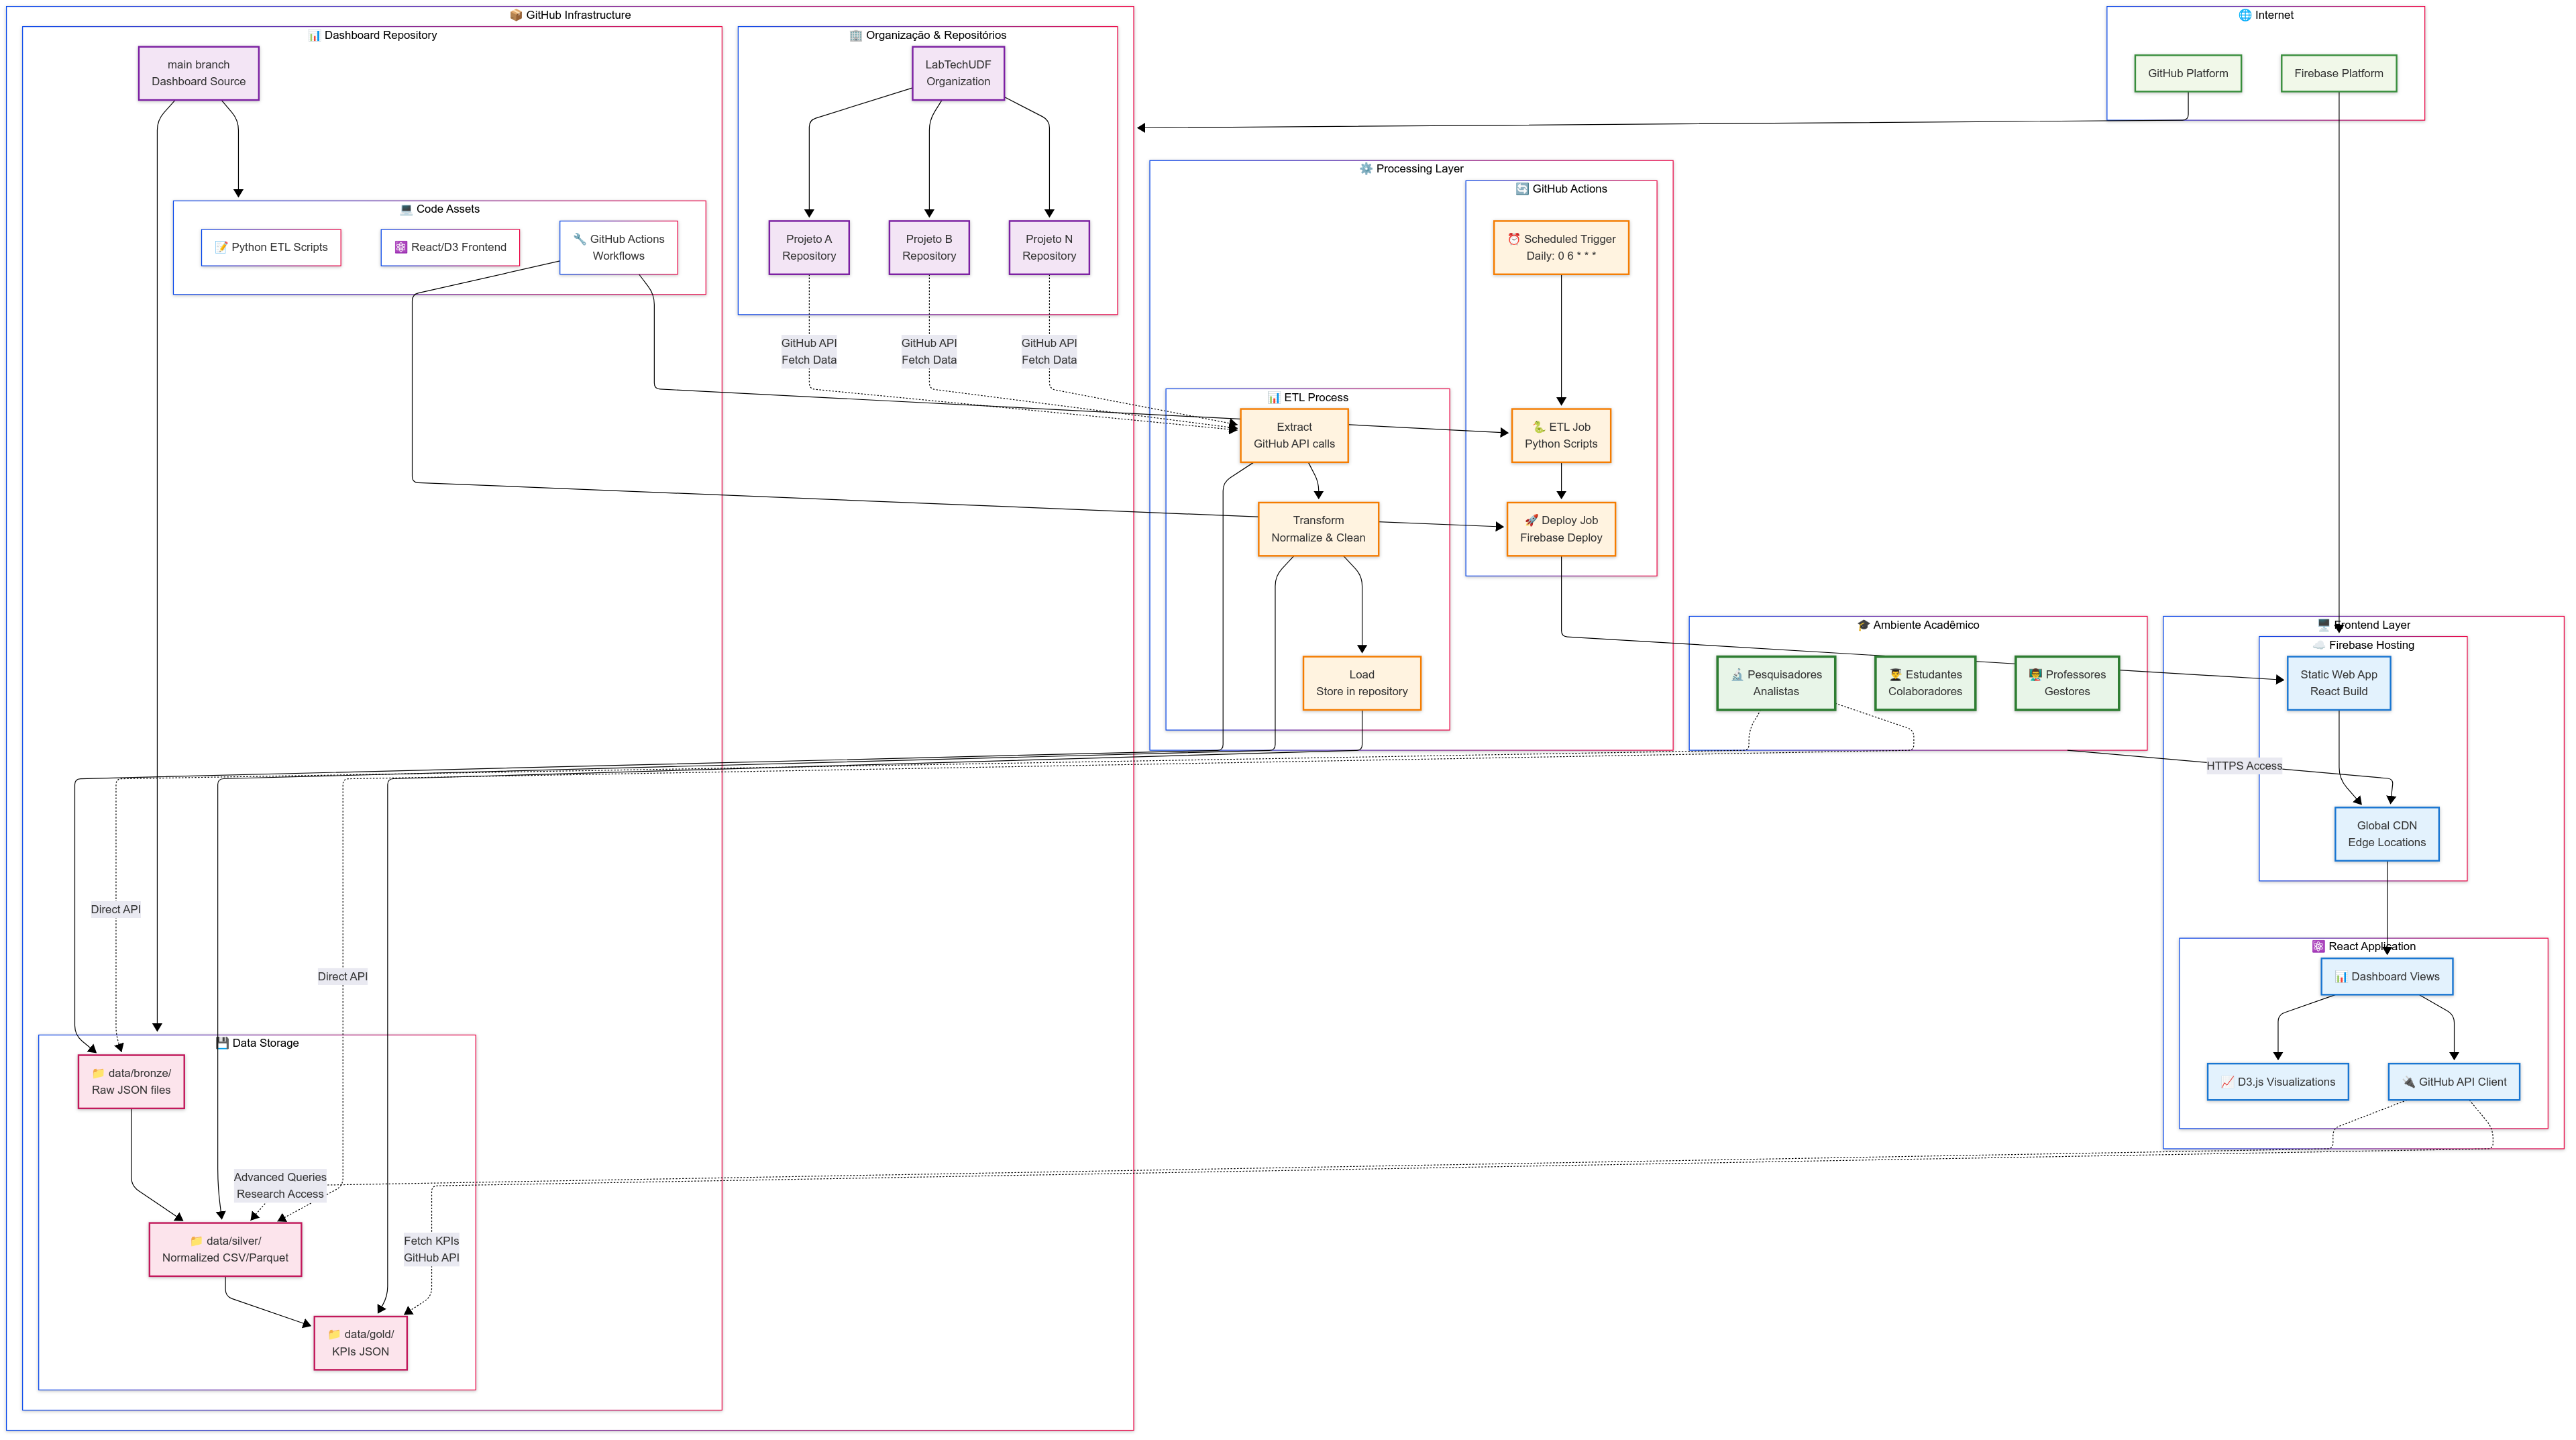
\includegraphics[width=0.85\textwidth]{arquitetura-geral.png}
\caption{Arquitetura geral do dashboard: solução serverless integrando GitHub Actions e GitHub Pages com React 19/D3.js}
\label{fig:arquitetura-geral}
\end{figure}

\subsection{Fluxo ETL e transformação de dados}
O processo ETL (Figura~\ref{fig:sequencia-etl}) opera em cinco fases principais:
\begin{enumerate}
    \item \textbf{Extração Bronze}: coleta via GitHub REST API com rate limiting e cache inteligente (7 módulos)
    \item \textbf{Transformação Silver}: normalização em 6 módulos analíticos
    \item \textbf{Agregação Gold}: cálculo de KPIs executivos e classificação de desempenho
    \item \textbf{Análise por IA}: geração de resumos em linguagem natural via API Google Gemini (opcional)
    \item \textbf{Deploy}: commit dos dados processados e deploy automático via GitHub Pages
\end{enumerate}

\textbf{Otimização de desempenho}: a migração de chamadas GraphQL para REST API resultou em ganho de \textbf{100x} no tempo de extração (de 3--4 horas para 30--40 segundos por organização), viabilizando a execução diária automatizada.

\begin{figure}[htbp]
\centering
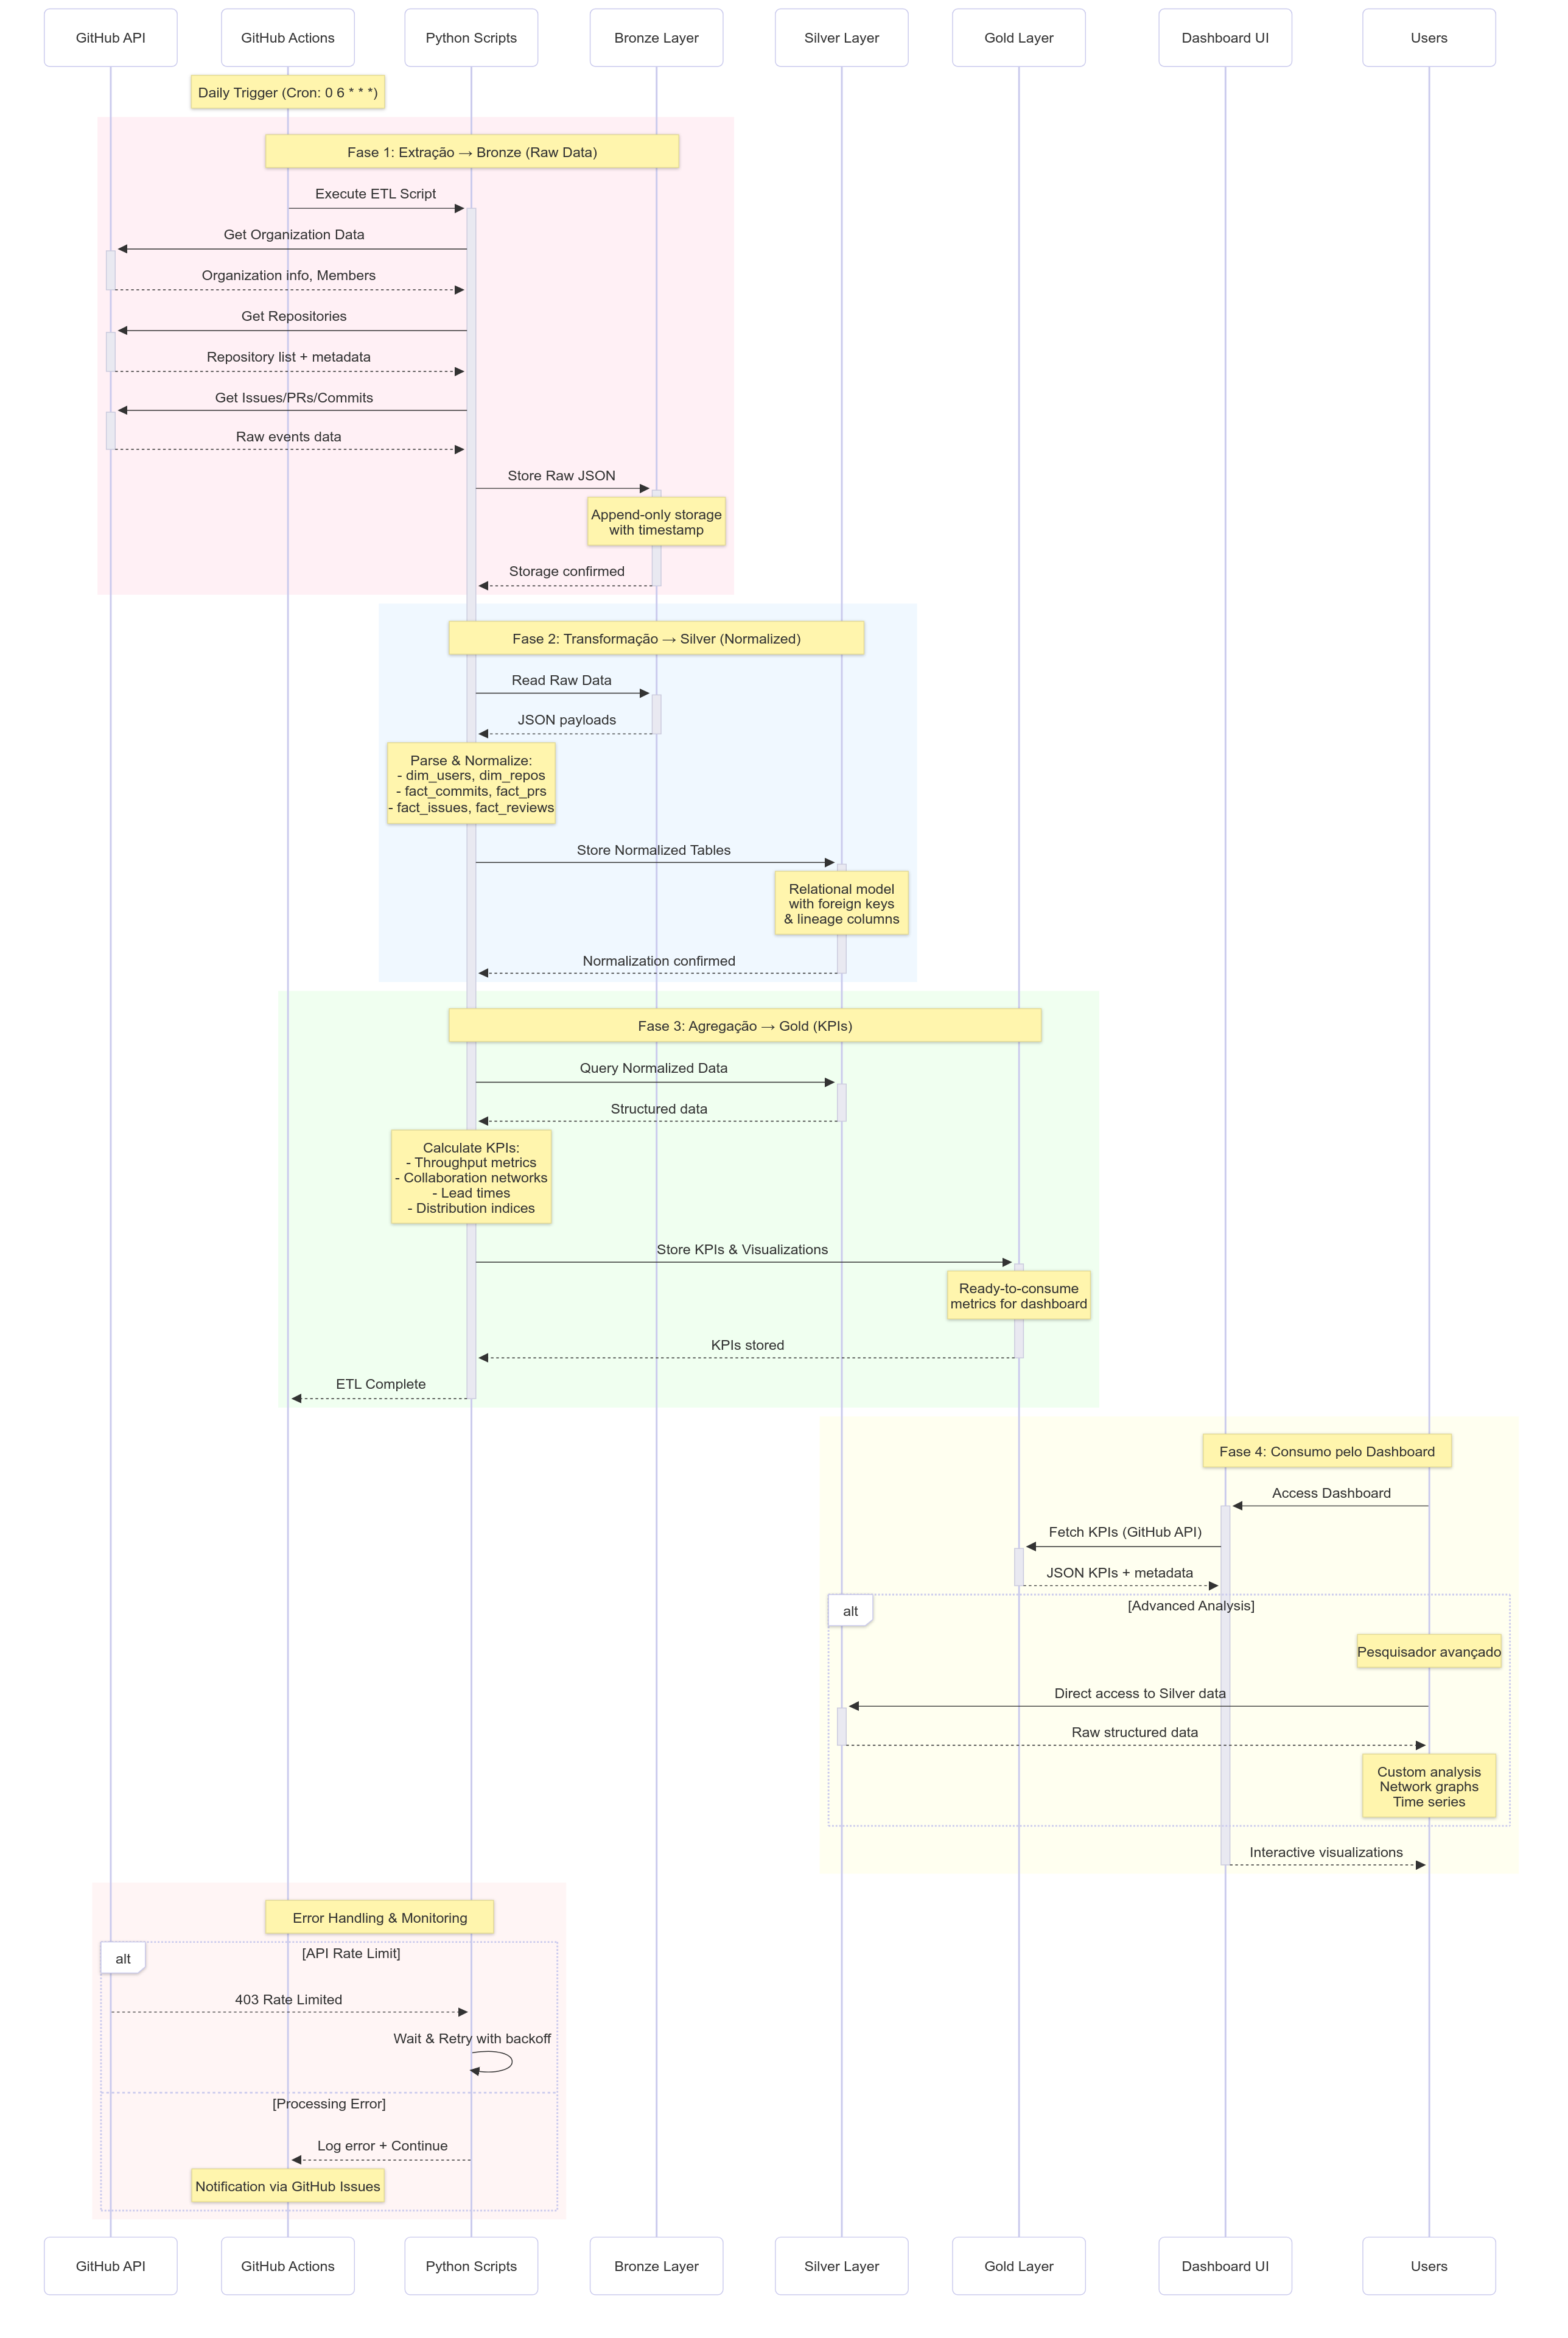
\includegraphics[width=0.85\textwidth]{sequencia_etl.png}
\caption{Diagrama de sequência do processo ETL automatizado via GitHub Actions}
\label{fig:sequencia-etl}
\end{figure}

\subsection{Pipeline de dados (Arquitetura Medalhão)}
A Figura~\ref{fig:dag-medalhao} ilustra o fluxo completo de dados da arquitetura medalhão implementada, desde as fontes GitHub API até as visualizações finais, passando pelas transformações Bronze$\rightarrow$Silver$\rightarrow$Gold.

\begin{figure}[htbp]
\centering
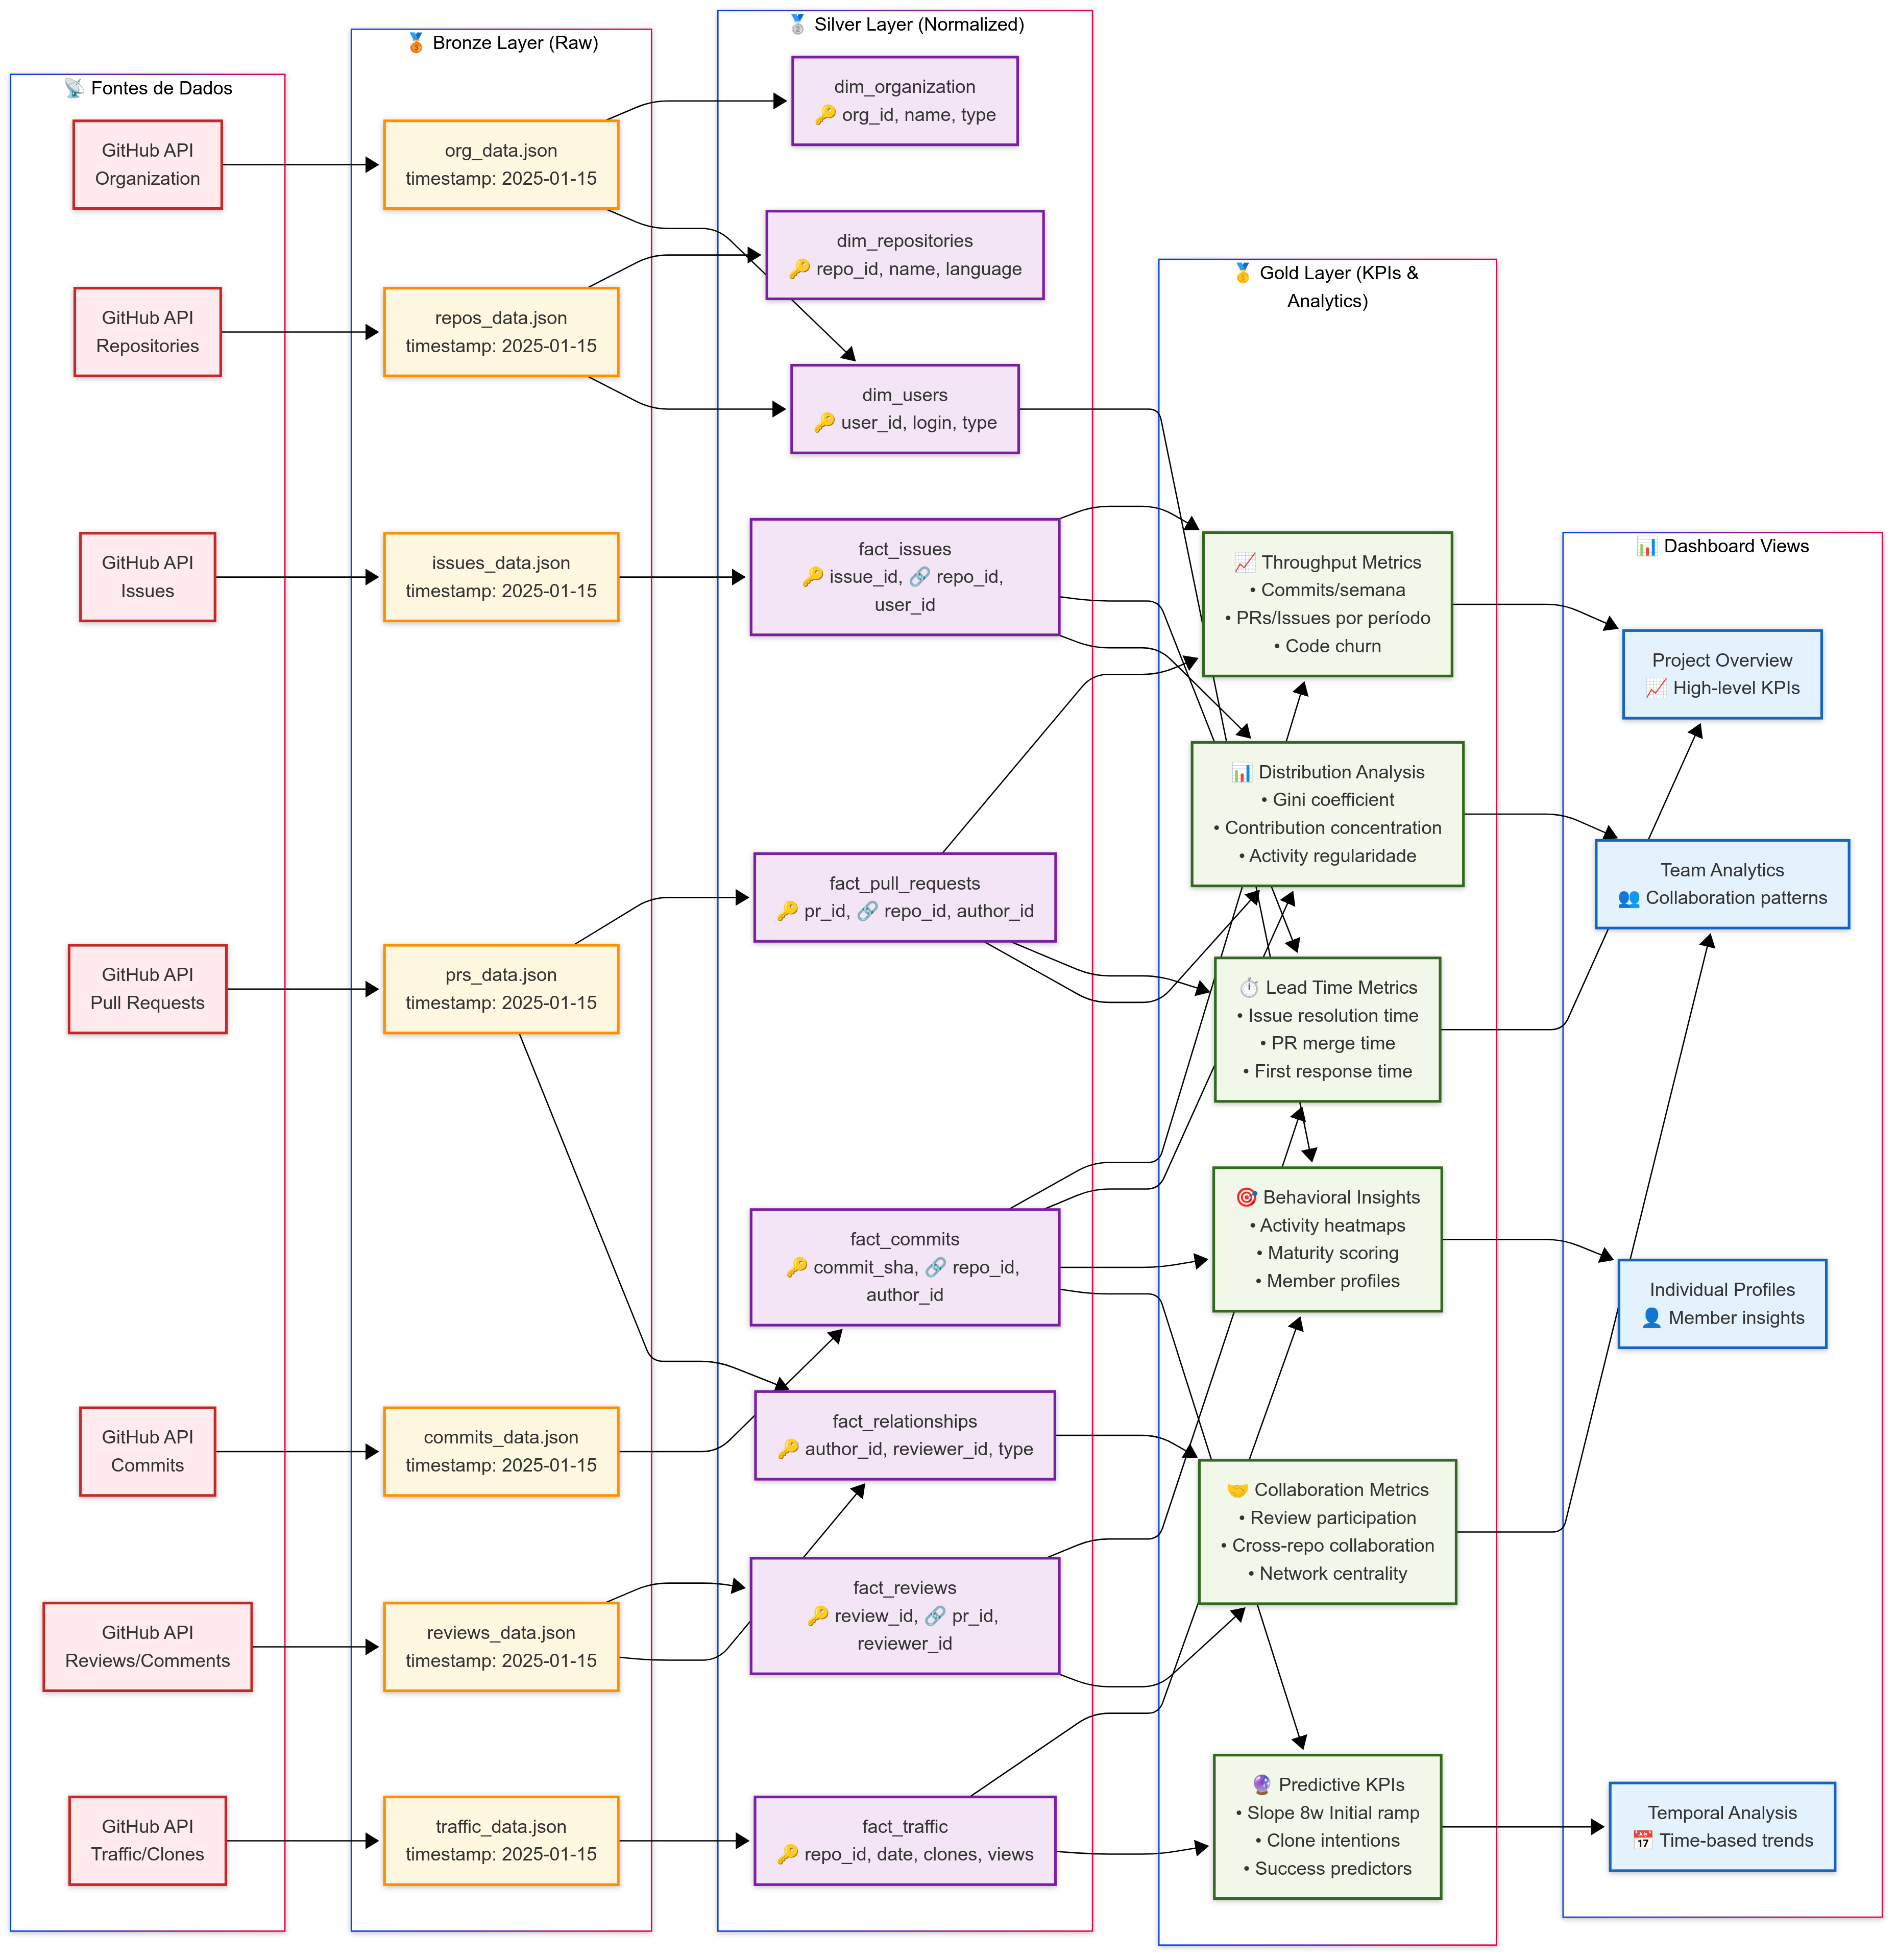
\includegraphics[width=0.9\textwidth]{dag-medalhao.png}
\caption{DAG da Arquitetura Medalhão: fluxo Bronze$\rightarrow$Silver$\rightarrow$Gold com todas as transformações de dados}
\label{fig:dag-medalhao}
\end{figure}

\subsection{Análise por inteligência artificial}

O dashboard integra a API do \textbf{Google Gemini} para geração de resumos em linguagem natural das contribuições de cada membro. O módulo opera com degradação graciosa: quando a API não está disponível, a plataforma funciona normalmente sem as análises por IA. Este módulo foi adicionado durante as iterações com Dra.\ Carla Rocha, atendendo à necessidade de interpretações contextuais dos dados quantitativos.

% ----------------------------------------------------------
% RESULTADOS
% ----------------------------------------------------------
\section{Resultados}

\subsection{Plataforma desenvolvida}

O dashboard é uma aplicação \textit{full-stack} de código aberto para análise cooperativa de organizações GitHub. Duas instâncias estão em produção:
\begin{itemize}
    \item \textbf{UnB (MDS)}: \url{https://unb-mds.github.io/2025-2-Squad-01/} --- analisa a organização \texttt{unb-mds} com 70+ repositórios.
    \item \textbf{UDF (LabTech)}: \url{https://labtechudf.github.io/CoOps/} --- analisa a organização \texttt{LabTechUDF}.
\end{itemize}

\begin{figure}[htbp]
\centering
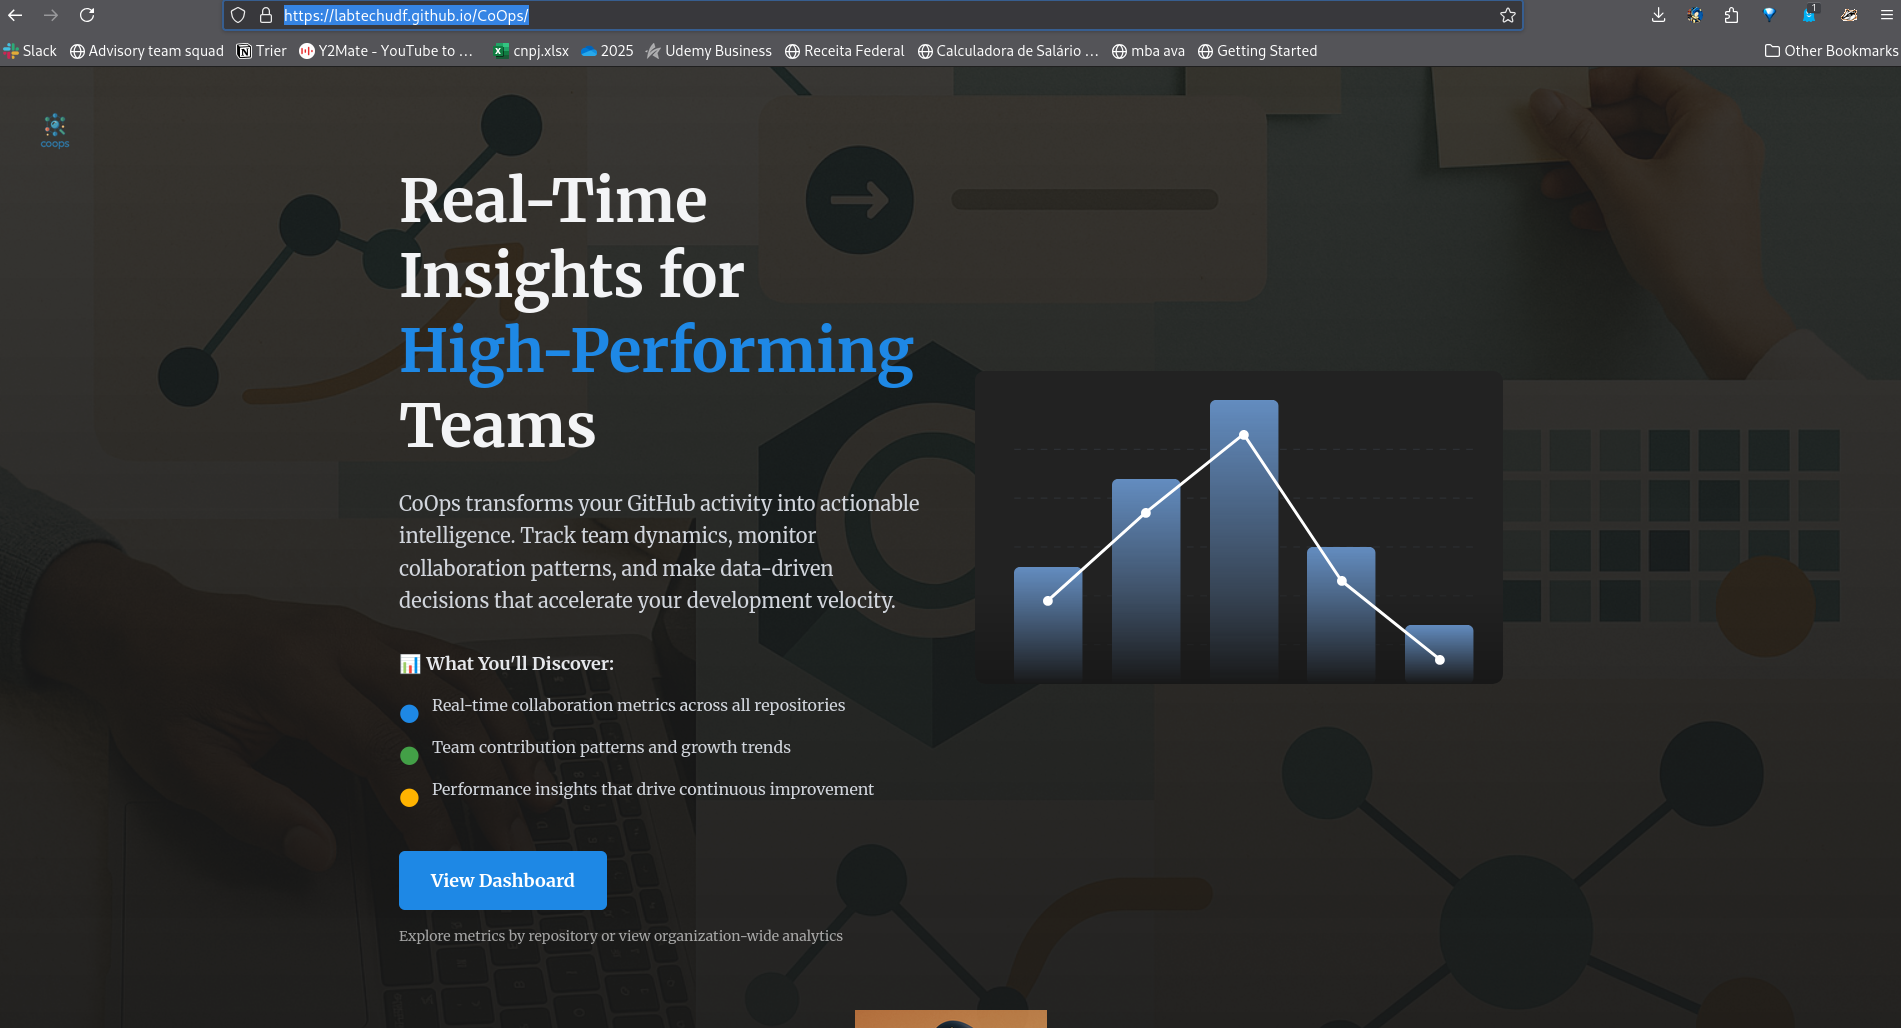
\includegraphics[width=0.85\textwidth]{screenshot-coops/pagina-inicial.png}
\caption{Página inicial do dashboard exibindo a visão geral da organização}
\label{fig:pagina-inicial}
\end{figure}

\subsection{Dashboard interativo: 13+ páginas com D3.js}

O frontend conta com \textbf{13+ páginas interativas} construídas com React 19 e D3.js:

\begin{itemize}
    \item \textbf{Treemap}: distribuição de repositórios por tamanho, atividade ou linguagem
    \item \textbf{CirclePack}: hierarquia de contribuições por membro e repositório
    \item \textbf{Rede de colaboração}: grafo interativo de interações entre membros
    \item \textbf{Activity Heatmap}: padrões temporais de atividade (dia $\times$ hora)
    \item \textbf{Timeline}: evolução temporal de métricas por repositório
    \item \textbf{Fingerprint de repositório}: análise de composição e estrutura de arquivos
    \item \textbf{Análise de commits}: frequência, distribuição e padrões por autor
    \item \textbf{Métricas de issues/PRs}: throughput, lead time, participação em revisões
    \item \textbf{KPIs executivos}: visão consolidada da organização com indicadores-chave
    \item \textbf{Distribuição de linguagens}: análise de composição tecnológica com suporte a 90+ tipos de arquivo
\end{itemize}

\begin{figure}[htbp]
\centering
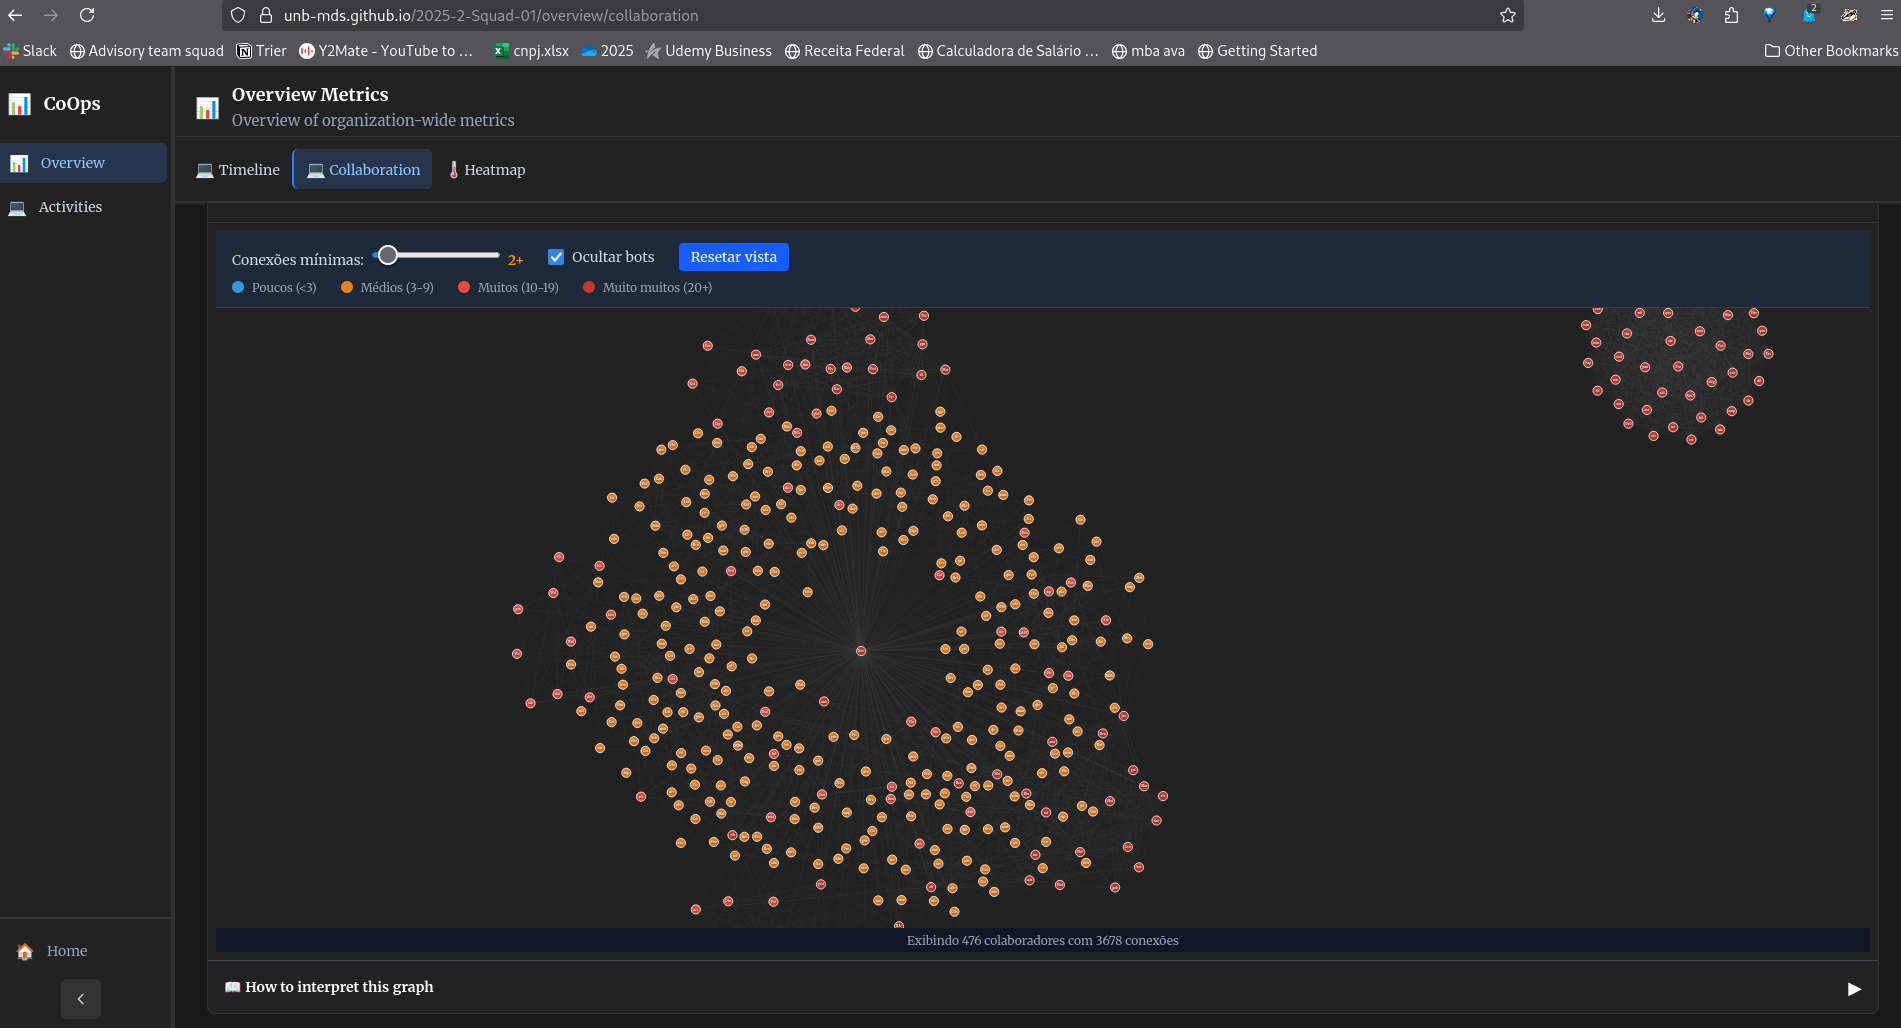
\includegraphics[width=0.85\textwidth]{screenshot-coops/rede-de-colaboracao.png}
\caption{Rede de colaboração interativa construída com D3.js, exibindo interações entre membros da organização}
\label{fig:rede-colaboracao}
\end{figure}

\begin{figure}[htbp]
\centering
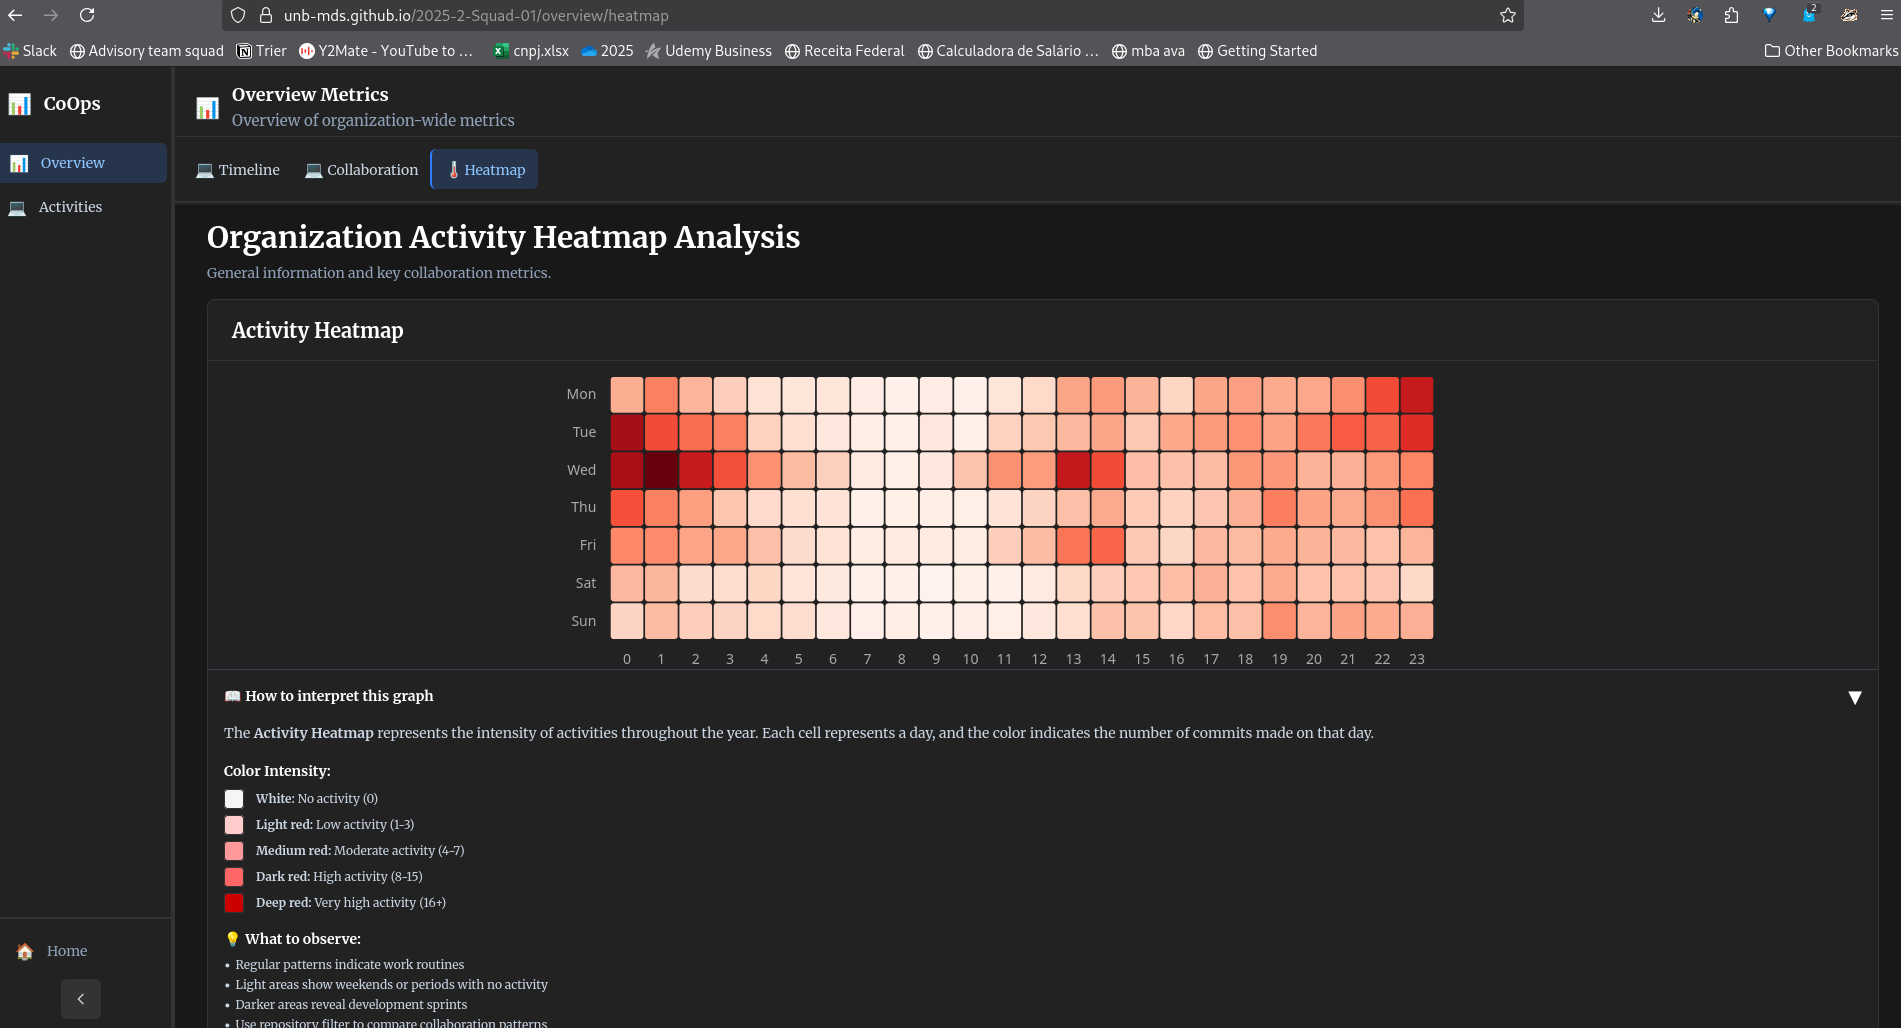
\includegraphics[width=0.85\textwidth]{screenshot-coops/heatmap.png}
\caption{Heatmap de atividade do dashboard: padrões temporais de contribuições}
\label{fig:heatmap}
\end{figure}

\begin{figure}[htbp]
\centering
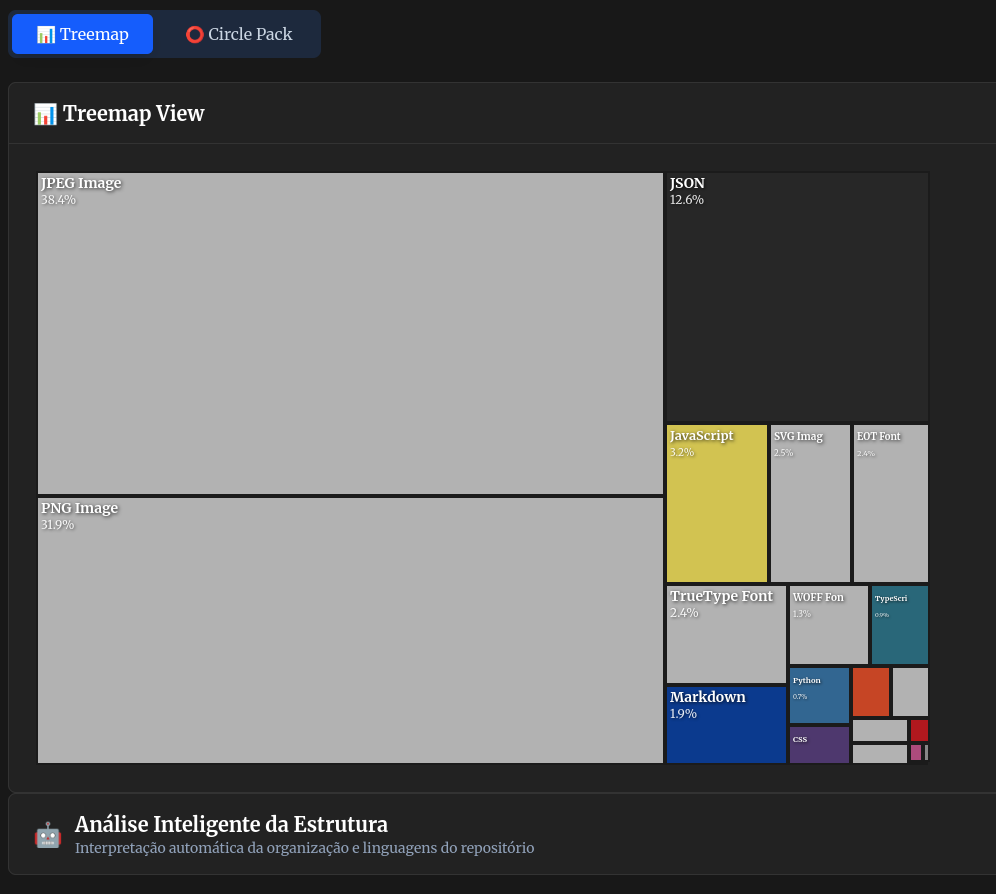
\includegraphics[width=0.85\textwidth]{screenshot-coops/treemap.png}
\caption{Visualização treemap dos repositórios da organização}
\label{fig:treemap}
\end{figure}

\begin{figure}[htbp]
\centering
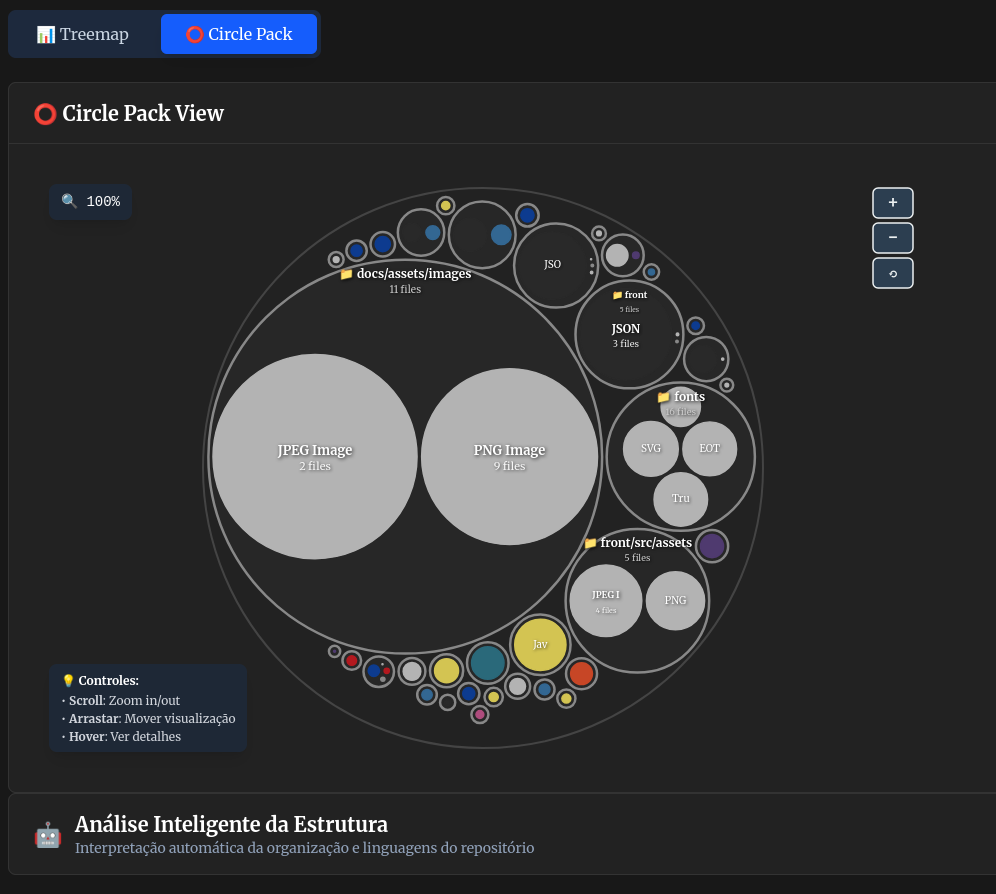
\includegraphics[width=0.85\textwidth]{screenshot-coops/circlepack-view.png}
\caption{Visualização CirclePack hierárquica de contribuições por membro e repositório}
\label{fig:circlepack}
\end{figure}

\subsection{Co-desenvolvimento e validação pedagógica real}

O modelo de co-desenvolvimento com Dra.\ Carla Rocha demonstrou-se eficaz:
\begin{itemize}
    \item Danrley construiu a plataforma e colaborou diretamente com Dra.\ Carla para definir quais dados Silver e Gold ela necessitava para suas disciplinas de MDS.
    \item O processo foi \textbf{iterativo}: a cada ciclo, novos módulos Silver/Gold eram implementados e validados.
    \item O módulo de \textbf{análise por IA} foi adicionado com base nas necessidades identificadas durante a colaboração.
    \item Ao final do semestre 2025/2, Dra.\ Carla \textbf{utilizou o dashboard para avaliar seus alunos} --- configurando uma validação pedagógica real do software.
    \item A instância UnB analisou \textbf{70+ repositórios} da organização \texttt{unb-mds}, demonstrando a escalabilidade da solução.
\end{itemize}

\begin{figure}[htbp]
\centering
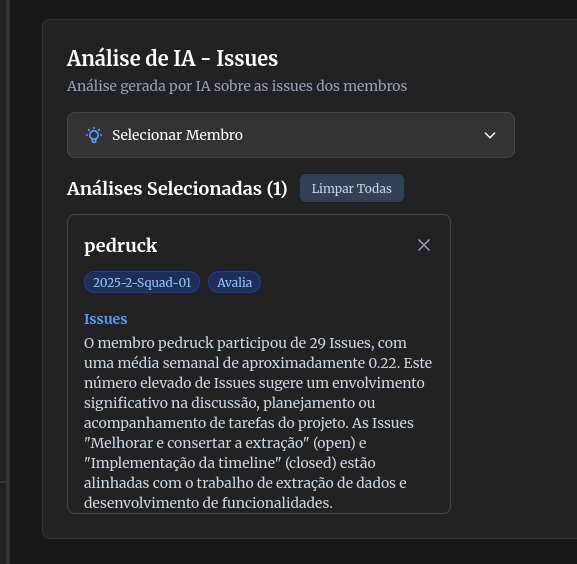
\includegraphics[width=0.85\textwidth]{screenshot-coops/ai-analysis-issues-from-one-member-from-mds.png}
\caption{Análise por IA (Google Gemini) das contribuições de um membro de equipe MDS}
\label{fig:ai-analysis}
\end{figure}

\begin{figure}[htbp]
\centering
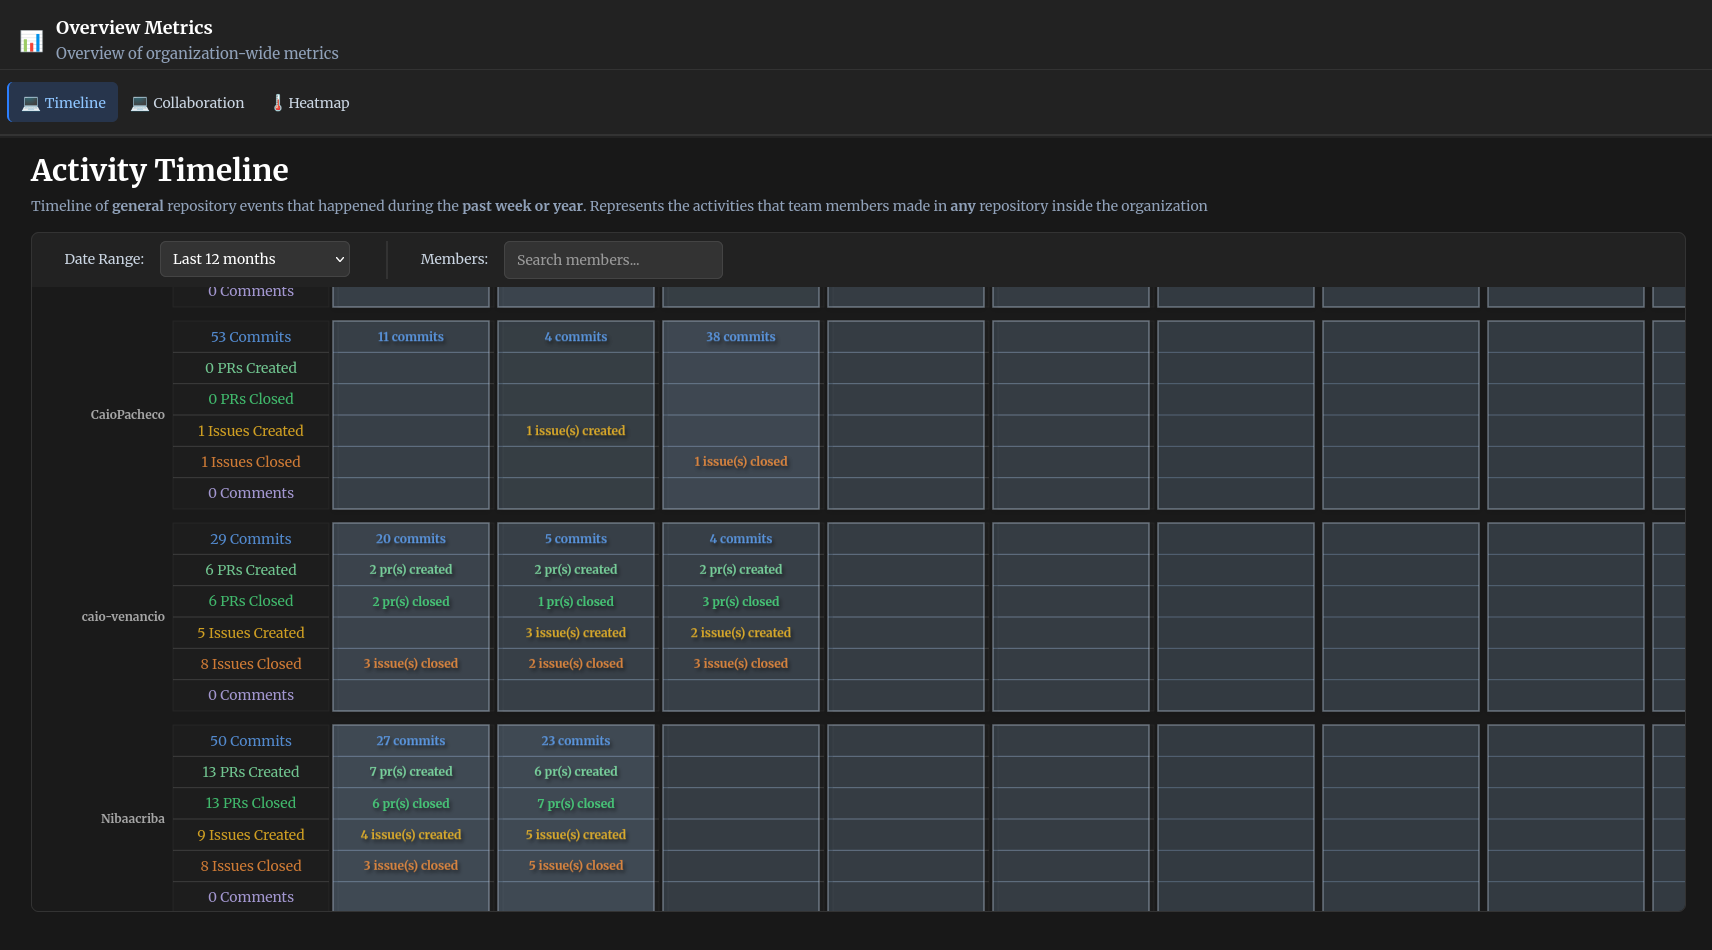
\includegraphics[width=0.85\textwidth]{screenshot-coops/activity-timeline-screen-partial-view-here-we-can-see-prs-issues-etc-by-user.png}
\caption{Timeline de atividade do dashboard analisando repositórios da organização unb-mds}
\label{fig:timeline-unb}
\end{figure}

\subsection{Pipeline de dados em produção}

O pipeline opera diariamente em produção via GitHub Actions, processando as três camadas da Arquitetura Medalhão de forma automatizada.

\begin{figure}[htbp]
\centering
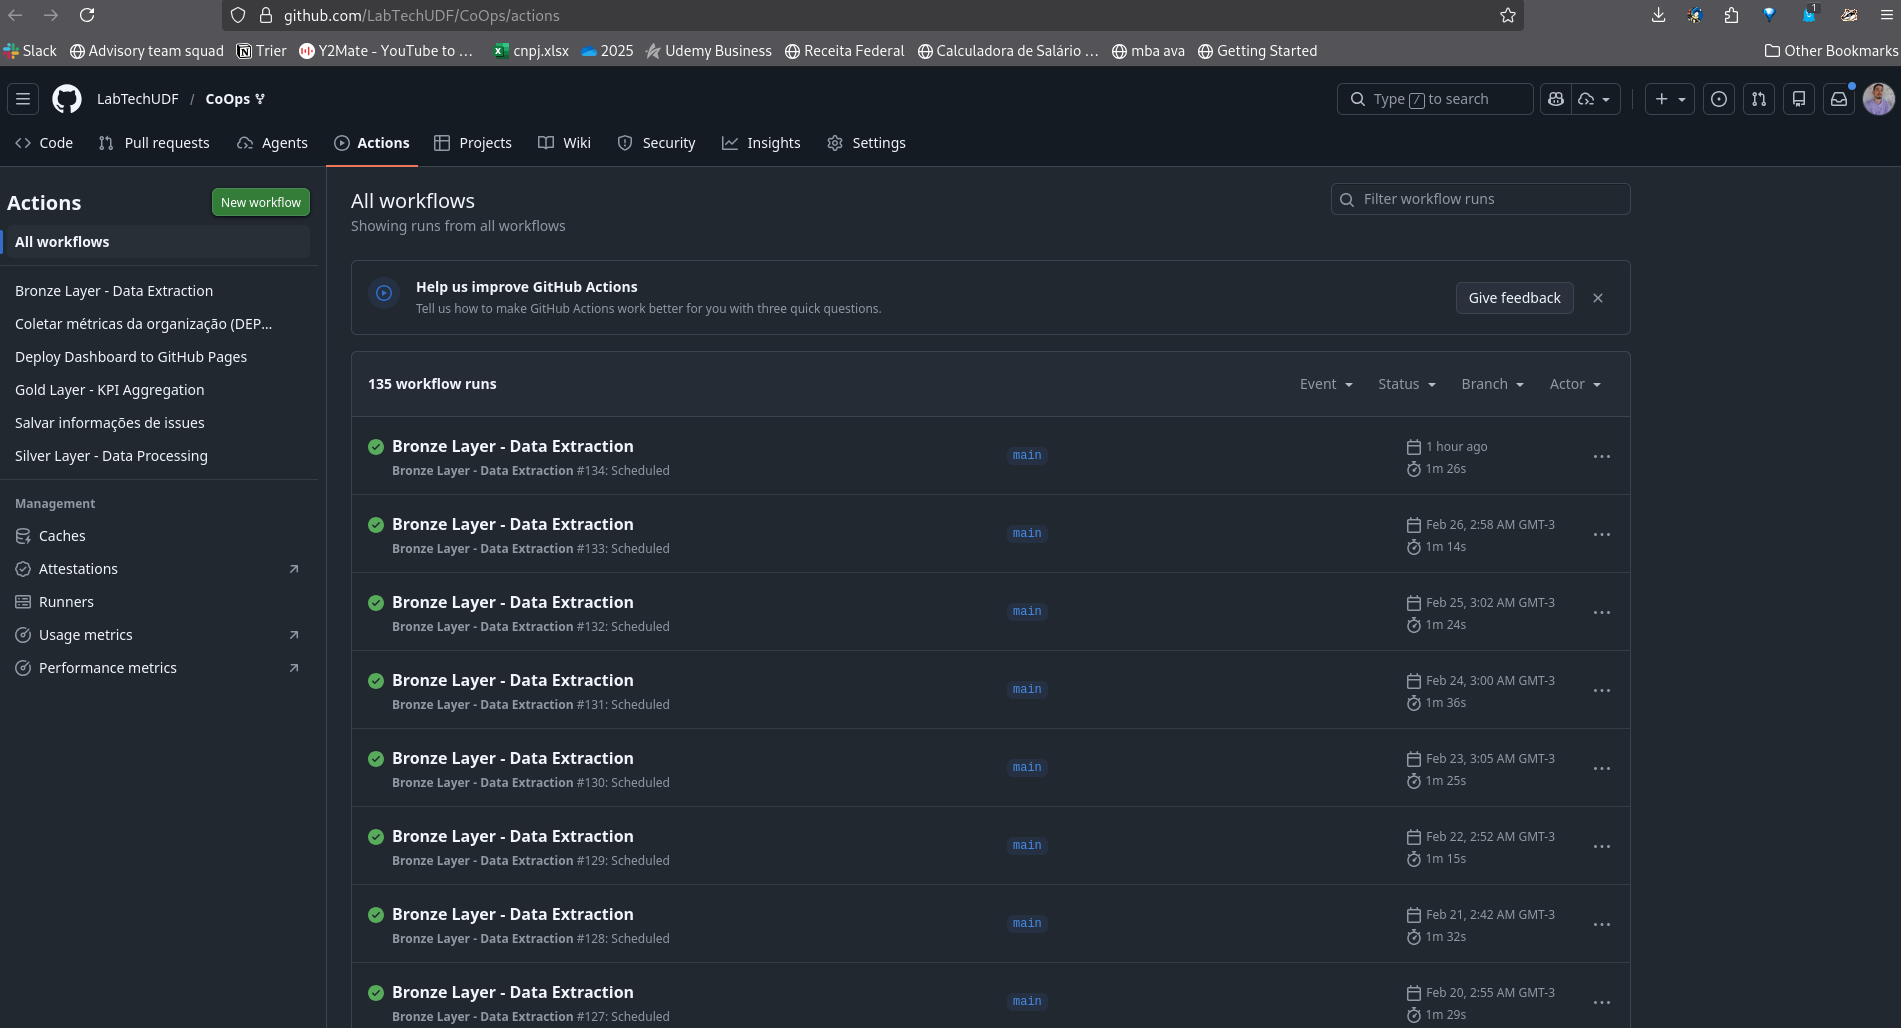
\includegraphics[width=0.85\textwidth]{screenshot-coops/pipelines-github-todos-workflows-rodados.png}
\caption{Workflows do GitHub Actions executando o pipeline de extração e transformação de dados do dashboard}
\label{fig:pipeline}
\end{figure}

\subsection{Testes e qualidade}

\begin{itemize}
    \item \textbf{Frontend}: \textbf{94\% de cobertura} de testes com Vitest + React Testing Library
    \item \textbf{Backend}: testes unitários e de integração com pytest
    \item \textbf{CI/CD}: GitHub Actions executa o pipeline diariamente às 5h UTC
    \item \textbf{Qualidade de código}: linting (ESLint, Ruff) integrado ao pipeline
\end{itemize}

\subsection{Validação qualitativa}

Os achados dos \textbf{Apêndices A e B} foram validados na prática com as turmas de Dra.\ Carla: (i) atualização semanal confirmou-se suficiente para governança pedagógica; (ii) grafos de colaboração efetivamente distinguem perfis integrador/especialista; (iii) métricas de ramp-up inicial e regularidade semanal são úteis para avaliação de alunos; (iv) a triangulação qualitativa-quantitativa fortalece a interpretação dos dados.

% ----------------------------------------------------------
% CONCLUSÃO
% ----------------------------------------------------------
\section{Conclusão}

Este trabalho apresentou o \textbf{Dashboard de Monitoramento} --- uma plataforma \textit{open source full-stack} que superou o escopo originalmente proposto, evoluindo de protótipos com 20 visualizações estáticas para uma aplicação em produção com 13+ páginas interativas D3.js, análise por IA e dois deployments ativos. O dashboard é alicerçado em: (i) \textbf{KPIs técnicos e colaborativos} implementados e validados; (ii) \textbf{Arquitetura Medalhão} completa (Bronze$\rightarrow$Silver$\rightarrow$Gold) com otimização de 100x; (iii) \textbf{triangulação} quanti-qualitativa (Apêndices A e B); (iv) \textbf{co-desenvolvimento} eficaz com Dra.\ Carla Rocha (UnB); e (v) \textbf{licença GPL v3.0} que democratiza o reuso.

A validação mais significativa foi o \textbf{uso real para avaliação de alunos} por Dra.\ Carla ao final do semestre, confirmando a relevância pedagógica do dashboard. A plataforma demonstra que práticas de engenharia de dados da indústria (Arquitetura Medalhão, CI/CD, deploy serverless) podem ser aplicadas com sucesso ao contexto acadêmico, operando com infraestrutura zero via GitHub Pages e GitHub Actions.

Como desdobramentos futuros, preveem-se: (a) expansão para mais instituições; (b) incorporação de métricas de qualidade de código (complexidade ciclomática, cobertura de testes dos projetos analisados); (c) predições baseadas em aprendizado de máquina para identificação precoce de equipes em risco; e (d) integração com outras plataformas além do GitHub.

% ----------------------------------------------------------
% Referências Bibliográficas
% ----------------------------------------------------------
\bibliography{artigo}

% ----------------------------------------------------------
% APÊNDICES
% ----------------------------------------------------------
\begin{apendicesenv}
\partapendices

\chapter{Entrevista com LAPPIS/UnB (FGA) --- Relatório de Reunião}
\label{apendiceA}

\textbf{Participantes:} Danrley Pereira (PIBIT/UDF) e Dra.\ Carla Rocha (Coordenadora LAPPIS) \\
\textbf{Data:} 22/08/2025 \\
\textbf{Local:} FGA -- UnB \\
\textbf{Tema:} Fábricas de software acadêmicas, métricas de interação e experiências do LAPPIS

\section*{1.\ Contexto Institucional}
\begin{itemize}
\item Envolvimento atual em \textbf{sistemas estruturantes} para controle orçamentário no poder executivo.
\item Desafio de \textbf{fragmentação de sistemas} e baixa interoperabilidade.
\end{itemize}

\section*{2.\ Reflexões sobre o modelo de ``Fábrica de Software''}
\begin{itemize}
\item Crítica ao conceito tradicional para ambientes acadêmicos/inovadores; necessidade de \textbf{repensar e adaptar} práticas ao aprendizado.
\end{itemize}

\section*{3.\ Arquitetura e tratamento de dados}
\begin{itemize}
\item Proposta da \textbf{Arquitetura Medalhão}:
\begin{itemize}
\item \textbf{Bronze (Raw):} extração de GitHub, GitLab, Notion;
\item \textbf{Silver:} transformação e homogeneização em modelos definidos;
\item \textbf{Gold:} camada de conhecimento com insights consolidados.
\end{itemize}
\item \textbf{Atualização semanal} considerada suficiente para o dashboard.
\end{itemize}

\section*{4.\ Métricas Quantitativas e Qualitativas}
\begin{itemize}
\item Necessidade de \textbf{interpretar quantitativos via análises qualitativas}.
\end{itemize}

\section*{5.\ Formação Acadêmica e Experiência}
\begin{itemize}
\item Disciplinas regulares: \textbf{4 meses}; alunos ingressam a partir do \textbf{4º semestre} e permanecem, em média, \textbf{2 anos}.
\end{itemize}

\section*{6.\ Métricas de Interações em Repositórios}
\begin{itemize}
\item Potencial de \textbf{grafos de rede} para mapear perfis:
\begin{itemize}
\item \textit{Aluno integrador}: muitos vínculos entre membros/repos;
\item \textit{Aluno especialista}: foco em áreas específicas (ex.: SRE/DevOps).
\end{itemize}
\end{itemize}

\section*{7.\ Conclusões e Próximos Passos}
\begin{itemize}
\item Alinhamento sobre utilidade de \textbf{métricas de interação} e adoção do modelo em \textbf{camadas (Bronze~$\rightarrow$~Silver~$\rightarrow$~Gold)}.
\item Reforço da \textbf{integração de contexto qualitativo} às análises.
\end{itemize}

\chapter{Relatos LABTECH/UDF --- Engajamento e Padrões de Contribuição}
\label{apendiceB}

\section*{Resumo dos relatos}
\begin{itemize}
\item No início do semestre, \textbf{interações no GitHub tendem a ser tímidas}, pois os alunos ainda estão se ambientando ao projeto e ao domínio.
\item A \textbf{curva inicial} pode ser mais baixa, com \textbf{aceleração ao redor da metade do semestre}.
\item \textbf{Commits e interações} mostram quem efetivamente contribuiu e buscou engajar.
\item O \textbf{número de \textit{clones}} no começo do semestre sinaliza a \textbf{intenção de participação}; acompanhar sua evolução pode indicar adesão.
\end{itemize}

\section*{Implicações para os KPIs}
\begin{itemize}
\item Monitorar a \textbf{inclinação inicial} (semanas 1--8) como possível preditor de sucesso posterior.
\item Persistir e analisar \textbf{clones} no início (\emph{traffic/clones}) como indicador de intenção.
\item Separar leituras por \textbf{papéis} (autor, revisor) e por \textbf{áreas} (dados, frontend, APIs, plataforma), permitindo distinguir \textit{integradores} de \textit{especialistas}.
\end{itemize}

\end{apendicesenv}

\end{document}
